\documentclass[lang=cn,newtx,10pt,scheme=chinese]{../../../elegantbook}

\title{基础提高练习题}
\subtitle{北街学长倾力之作}

\author{北街}
% \institute{Elegant\LaTeX{} Program}
\date{2022/12/31}
\version{1.0}
% \bioinfo{自定义}{信息}

% \extrainfo{注意:本模板自 2023 年 1 月 122222 日开始,不再更新和维护!}

\setcounter{tocdepth}{3}

\logo{../../figure/logo-blue.png}
\cover{../../figure/cover.jpg}

% 本文档命令
\usepackage{array}
\newcommand{\ccr}[1]{\makecell{{\color{#1}\rule{1cm}{1cm}}}}

% 修改标题页的橙色带
\definecolor{customcolor}{RGB}{32,178,170}
\colorlet{coverlinecolor}{customcolor}
\usepackage{cprotect}

\addbibresource[location=local]{reference.bib} % 参考文献,不要删除
\usepackage{listings}         % 导入listings宏包
\usepackage{xcolor}           % 支持颜色

% 配置C++代码样式
\lstset{
    language=C++,             % 语言设置为C++
    basicstyle=\ttfamily,      % 基本样式
    keywordstyle=\color{blue}, % 关键词颜色
    commentstyle=\color{green},% 注释颜色
    stringstyle=\color{red},   % 字符串颜色
    numbers=left,              % 显示行号
    numberstyle=\tiny,         % 行号样式
    stepnumber=1,              % 每行显示行号
    breaklines=true,           % 自动换行
    frame=lines                % 代码块边框样式
}
\begin{document}

\maketitle
\frontmatter

\tableofcontents

\mainmatter


\chapter{树与二叉树}


\begin{enumerate}
        \item 若将一棵树 $T$ 转化为对应的二叉树 $BT$,则下列对 $BT$ 的遍历中,其遍历序列与 $T$ 的后根遍历序列相同的是( )。  
        【2019 年全国试题 2(2 分)】  
    
        A. 先序遍历 \quad B. 中序遍历 \quad C. 后序遍历 \quad D. 按层遍历  
    
        答案:\textcolor{red}{C}
        
        解析:\\
        将树转换为二叉树的规则是:每个结点的左孩子是其在树中的第一个孩子,右孩子是其在树中的下一个兄弟。\\
        在这种转换下:\\
        1. 树的先根遍历对应二叉树的先序遍历\\
        2. 树的后根遍历对应二叉树的后序遍历\\
        3. 树的层次遍历与二叉树的层次遍历不对应\\
        因此,树 $T$ 的后根遍历序列与其对应的二叉树 $BT$ 的后序遍历序列相同。\\
    
        \item 对 $n$ 个互不相同的符号进行哈夫曼编码。若生成的哈夫曼树共有 115 个结点,则 $n$ 的值是( )。  
        【2019 年全国试题 3(2 分)】  
    
        A. 56 \quad B. 57 \quad C. 58 \quad D. 60  
    
        答案:\textcolor{red}{C}
        
        解析:\\
        在哈夫曼树中,若有 $n$ 个叶子结点(即 $n$ 个符号),则树中共有 $2n-1$ 个结点。\\
        这是因为:\\
        1. 初始有 $n$ 个结点(叶子结点)\\
        2. 每次合并两个结点生成一个新结点,共进行 $n-1$ 次合并\\
        3. 因此总结点数为 $n + (n-1) = 2n-1$\\
        
        已知哈夫曼树共有 115 个结点,则:\\
        $2n-1 = 115$\\
        $2n = 116$\\
        $n = 58$\\
        
        因此,$n$ 的值是 58。\\
    
        \item 设一棵非空完全二叉树 $T$ 的所有叶结点均位于同一层,且每个非叶结点都有 2 个子结点。若 $T$ 有 $m$ 个叶结点,则 $T$ 的结点总数是( )。  
        【2018 年全国试题 4(2 分)】
    
        A. $2m - 1$ \quad B. $2m$ \quad C. $m^2$ \quad D. $2^{m} - 1$  
    
        答案:\textcolor{red}{A}
        
        解析:\\
        这棵树实际上是一棵满二叉树,因为所有叶结点均位于同一层,且每个非叶结点都有 2 个子结点。\\
        
        在满二叉树中,若树的高度为 $h$(根结点所在层为第 1 层),则:\\
        1. 叶结点数为 $2^{h-1}$\\
        2. 总结点数为 $2^h - 1$\\
        
        已知叶结点数为 $m$,即 $m = 2^{h-1}$\\
        则总结点数为 $2^h - 1 = 2 \times 2^{h-1} - 1 = 2m - 1$\\
        
        因此,$T$ 的结点总数是 $2m - 1$。\\
    
        \item 已知字符集 $\{a, b, c, d, e, f\}$,若各字符出现的次数分别为 $6, 3, 8, 2, 10, 4$,则对应字符集中各字符的哈夫曼编码可能是( )。  
        【2018 年全国试题 5(2 分)】  
    
        A. $00, 1011, 01, 1010, 11, 100$  
    
        B. $00, 100, 110, 000, 0010, 01$  
    
        C. $10, 1011, 11, 0011, 00, 010$  
    
        D. $0011, 10, 11, 0010, 01, 000$  
    
        答案:\textcolor{red}{C}
        
        解析:\\
        构建哈夫曼树时,首先按照权值(出现次数)从小到大排序:$d(2), b(3), f(4), a(6), c(8), e(10)$\\
        
        在哈夫曼编码中,权值小的结点通常位于树的较深层,编码较长;权值大的结点位于较浅层,编码较短。\\
        
        检查各选项:\\
        A选项:$00(a), 1011(b), 01(c), 1010(d), 11(e), 100(f)$\\
        这里 $a(6)$ 的编码比 $e(10)$ 短,不符合哈夫曼编码特性。\\
        
        B选项:$00(a), 100(b), 110(c), 000(d), 0010(e), 01(f)$\\
        这里 $e(10)$ 的编码比 $a(6)$ 长,不符合哈夫曼编码特性。\\
        
        C选项:$10(a), 1011(b), 11(c), 0011(d), 00(e), 010(f)$\\
        权值最大的 $e(10)$ 编码最短为 $00$,权值最小的 $d(2)$ 和 $b(3)$ 编码最长,符合哈夫曼编码特性。\\
        
        D选项:$0011(a), 10(b), 11(c), 0010(d), 01(e), 000(f)$\\
        这里 $b(3)$ 的编码比 $a(6)$ 短,不符合哈夫曼编码特性。\\
        
        因此,C选项符合哈夫曼编码的特性。\\
    
        \item 要使一棵非空二叉树的先序序列与中序序列相同,其所有非叶结点需满足的条件是( )。  
        【2017 年全国试题 4(2 分)】  
    
        A. 只有左子树  
    
        B. 只有右子树  
    
        C. 结点的度均为 1  
    
        D. 结点的度均为 2  
    
        答案:\textcolor{red}{A}
        
        解析:\\
        先序遍历的顺序是:根结点 → 左子树 → 右子树\\
        中序遍历的顺序是:左子树 → 根结点 → 右子树\\
        
        要使先序序列与中序序列相同,必须保证根结点在先序和中序中的位置相同。\\
        
        如果一个非叶结点有右子树,那么在先序遍历中,右子树中的结点会在左子树之后访问;而在中序遍历中,右子树中的结点会在根结点之后访问。这会导致先序序列和中序序列不同。\\
        
        因此,要使先序序列与中序序列相同,所有非叶结点必须只有左子树,没有右子树。\\
        
        所以,答案是 A. 只有左子树。\\
    
        \item 已知一棵二叉树的树形如下图所示,其后序序列为 $e, a, c, b, d, g, f$,树中与结点 $g$ 同层的结点是( )。  
        【2017 年全国试题 5(2 分)】  
    
        \begin{figure}[h!]
                \centering
                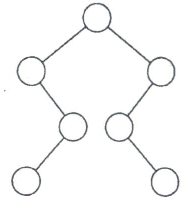
\includegraphics[width=0.3\textwidth]{../../figure/exercisePicPDF/chapter6/6-6.pdf}
                \caption{二叉树示意图}
        \end{figure}
    
        A. $c$  
    
        B. $d$  
    
        C. $f$  
    
        D. $g$  
    
        答案:\textcolor{red}{B}
        
        解析:\\
        根据后序遍历序列 $e, a, c, b, d, g, f$ 和图中的二叉树结构,我们可以确定:\\
        1. $f$ 是根结点\\
        2. $g$ 是 $f$ 的右子结点\\
        3. $d$ 是 $f$ 的左子结点\\
        4. $b$ 是 $d$ 的右子结点\\
        5. $c$ 是 $b$ 的左子结点\\
        6. $a$ 是 $d$ 的左子结点\\
        7. $e$ 是 $a$ 的左子结点\\
        
        从树的层次结构看,$f$ 在第一层,$d$ 和 $g$ 在第二层,$a$ 和 $b$ 在第三层,$e$ 和 $c$ 在第四层。\\
        
        因此,与结点 $g$ 同层的结点是 $d$。\\
    
        \item 已知字符集 $\{a, b, c, d, e, f, g, h\}$,若各字符的哈夫曼编码依次是 $0100, 10, 0000, 0101, 001, 011, 11, 0001$,则编码序列 $0100011001001011110101$ 的译码结果是( )。  
        【2017 年全国试题 6(2 分)】  
    
        A. $acgabfh$  
    
        B. $adbagbb$  
    
        C. $afbeagd$  
    
        D. $afeefgd$  
    
        答案:\textcolor{red}{C}
        
        解析:\\
        根据给定的哈夫曼编码:\\
        $a: 0100$\\
        $b: 10$\\
        $c: 0000$\\
        $d: 0101$\\
        $e: 001$\\
        $f: 011$\\
        $g: 11$\\
        $h: 0001$\\
        
        对编码序列 $0100011001001011110101$ 进行译码:\\
        $0100 \rightarrow a$\\
        $011 \rightarrow f$\\
        $10 \rightarrow b$\\
        $001 \rightarrow e$\\
        $10 \rightarrow b$\\
        $11 \rightarrow g$\\
        $0101 \rightarrow d$\\
        
        因此,译码结果是 $afbeagd$,对应选项 C。\\
    
        \item 若森林已知有 15 条边、25 个结点,则森林包含树的个数是( )。  
        【2016 年全国试题 5(2 分)】 
    
        A. 8 \quad B. 9 \quad C. 10 \quad D. 11  
    
        答案:\textcolor{red}{C}
        
        解析:\\
        在一棵有 $n$ 个结点的树中,边的数量为 $n-1$。\\
        
        对于包含 $k$ 棵树的森林,如果总共有 $N$ 个结点和 $E$ 条边,则有:\\
        $E = N - k$\\
        
        已知森林有 15 条边、25 个结点,则:\\
        $15 = 25 - k$\\
        $k = 25 - 15 = 10$\\
        
        因此,森林包含 10 棵树。\\
    
        \item 给定二叉树如下图所示。设 $W$ 代表二叉树的根,$L$ 代表根结点的左子树,$R$ 代表根结点的右子树。若遍历后的结点序列为 $3, 1, 7, 5, 6, 2, 4$,则其遍历方式是( )。  
        【2009 年全国试题 3(2 分)】  
    
        \begin{figure}[h!]
                \centering
                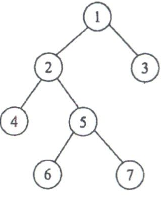
\includegraphics[width=0.3\textwidth]{../../figure/exercisePicPDF/chapter6/6-9.pdf}
                \caption{二叉树示意图}
        \end{figure}
    
        A. $LRN$ \quad B. $NRL$ \quad C. $RLN$ \quad D. $RNL$  
    
        答案:\textcolor{red}{C}
        
        解析:\\
        根据图中的二叉树结构,我们可以确定:\\
        - 根结点 $W$ 是 4\\
        - 左子树 $L$ 包含结点 1、3\\
        - 右子树 $R$ 包含结点 2、5、6、7\\
        
        遍历序列为 $3, 1, 7, 5, 6, 2, 4$\\
        
        分析各选项:\\
        A. $LRN$(左子树 → 右子树 → 根):应该是 $L$ 的遍历结果 + $R$ 的遍历结果 + 4,不符合给定序列\\
        
        B. $NRL$(根 → 右子树 → 左子树):应该是 4 + $R$ 的遍历结果 + $L$ 的遍历结果,不符合给定序列\\
        
        C. $RLN$(右子树 → 左子树 → 根):$R$ 的遍历结果 + $L$ 的遍历结果 + 4\\
        如果 $R$ 的遍历结果是 $3, 1$,$L$ 的遍历结果是 $7, 5, 6, 2$,则完整序列为 $3, 1, 7, 5, 6, 2, 4$,符合给定序列\\
        
        D. $RNL$(右子树 → 根 → 左子树):应该是 $R$ 的遍历结果 + 4 + $L$ 的遍历结果,不符合给定序列\\
        
        因此,遍历方式是 C. $RLN$(右子树 → 左子树 → 根)。\\
    
        \item 已知一棵完全二叉树的第 6 层(设根是第 1 层)有 8 个叶结点,则该完全二叉树的结点个数最多是( )。  
        【2009 年全国试题 5(2 分)】  
    
        A. 39 \quad B. 52 \quad C. 111 \quad D. 119  
    
        答案:\textcolor{red}{D}
        
        解析:\\
        在完全二叉树中,如果第 $h$ 层有叶结点,那么第 1 到第 $h-1$ 层都是满的,且第 $h$ 层的结点从左到右连续排列。\\
        
        已知第 6 层有 8 个叶结点,说明第 6 层共有 8 个结点,且都是叶结点。\\
        
        第 6 层最多可以有 $2^{6-1} = 2^5 = 32$ 个结点,现在只有 8 个,说明第 6 层不是满的。\\
        
        由于完全二叉树的性质,第 6 层的 8 个叶结点必须是从左到右连续排列的。\\
        
        计算结点总数:\\
        1. 第 1 到第 5 层的结点数:$2^1 - 1 + 2^2 - 2^1 + 2^3 - 2^2 + 2^4 - 2^3 + 2^5 - 2^4 = 2^5 - 1 = 31$\\
        2. 第 6 层的结点数:由于第 6 层有 8 个叶结点,且完全二叉树中第 6 层的非叶结点必须有两个子结点,这意味着第 7 层必须有 $(32-8) \times 2 = 48$ 个结点\\
        3. 第 7 层的结点数:48\\
        4. 第 8 层的结点数:0\\
        
        因此,结点总数为 $31 + 32 + 48 = 111$\\
        
        但是,题目问的是"结点个数最多是多少",考虑到完全二叉树的定义,第 7 层可能还有 8 个结点(对应第 6 层最右边的 4 个非叶结点的右子结点),所以最多可能有 $111 + 8 = 119$ 个结点。\\
        
        因此,该完全二叉树的结点个数最多是 119。\\
    
        \item 将森林转换为对应的二叉树,若在二叉树中,结点 $z$ 是结点 $y$ 的父结点的父结点,则在原来的森林中,$z$ 和 $y$ 可能具有的关系是( )。  
        
        I. 父子关系  
    
        II. 兄弟关系  
    
        III. z 的父结点与 y 的父结点是兄弟关系  
    
        A. 只有 II  
    
        B. I 和 II  
    
        C. I 和 III  
    
        D. I 、II 和 III  
    
        答案:\textcolor{red}{C}
        
        解析:\\
        将森林转换为二叉树的规则是:\\
        1. 每个结点的左孩子是其在原森林中的第一个孩子\\
        2. 每个结点的右孩子是其在原森林中的下一个兄弟\\
        
        若在二叉树中,结点 $z$ 是结点 $y$ 的父结点的父结点,则有以下可能的关系:\\
        
        I. 父子关系:\\
        如果 $y$ 是 $z$ 的孙子(即 $y$ 是 $z$ 的某个孩子的孩子),那么在转换为二叉树后,$y$ 可能是 $z$ 的左孩子的左孩子。这种情况下,在原森林中,$z$ 和 $y$ 是父子关系。\\
        
        II. 兄弟关系:\\
        如果 $z$ 和 $y$ 在原森林中是兄弟关系,那么在转换为二叉树后,$z$ 应该是 $y$ 的某个祖先的右孩子,而不是 $y$ 的父结点的父结点。因此,这种关系不可能。\\
        
        III. $z$ 的父结点与 $y$ 的父结点是兄弟关系:\\
        如果 $z$ 的父结点和 $y$ 的父结点在原森林中是兄弟关系,那么在转换为二叉树后,$z$ 的父结点可能是 $y$ 的父结点的右兄弟,这样 $z$ 就可能是 $y$ 的父结点的父结点的左孩子的右孩子。这种情况下,在原森林中,$z$ 的父结点与 $y$ 的父结点是兄弟关系。\\
        
        因此,可能的关系是 I 和 III,答案是 C。\\
    
        \item 下列线索二叉树中(用虚线表示线索),符合后序线索树定义的是( )。  
        【2010 年全国试题 3(2 分)】  
    
        \begin{figure}[h!]
                \centering
                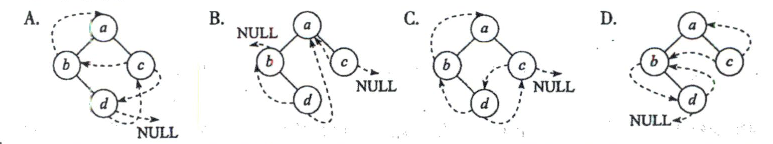
\includegraphics[width=1\textwidth]{../../figure/exercisePicPDF/chapter6/6-12.pdf}
                \caption{线索二叉树示意图}
        \end{figure}
    
        答案:\textcolor{red}{D}
        
        解析:\\
        后序线索二叉树是指按照后序遍历的顺序建立线索的二叉树。在后序线索二叉树中:\\
        1. 如果结点的左孩子指针为空,则该指针指向后序遍历中的前驱结点\\
        2. 如果结点的右孩子指针为空,则该指针指向后序遍历中的后继结点\\
        
        分析各选项:\\
        A图:结点 c 的右孩子指针为空,应该指向其后序遍历的后继结点 d,但图中指向了 b,不符合后序线索树定义\\
        
        B图:结点 c 的左孩子指针为空,应该指向其后序遍历的前驱结点,但图中指向了 d,不符合后序线索树定义\\
        
        C图:结点 c 的右孩子指针为空,应该指向其后序遍历的后继结点 a,但图中指向了 b,不符合后序线索树定义\\
        
        D图:按照后序遍历顺序,遍历序列为 c, d, b, e, a\\
        - 结点 c 的左孩子指针为空,指向其前驱结点(在后序遍历中 c 是第一个结点,没有前驱)\\
        - 结点 c 的右孩子指针为空,指向其后继结点 d\\
        - 结点 e 的左孩子指针为空,指向其前驱结点 b\\
        - 结点 e 的右孩子指针为空,指向其后继结点 a\\
        符合后序线索树定义\\
        
        因此,符合后序线索树定义的是 D。\\
    

        \item 在一棵度为 4 的树 $T$ 中,若有 20 个度为 4 的结点,10 个度为 3 的结点,1 个度为 2 的结点,10 个度为 1 的结点,则树 $T$ 的叶结点个数是( )。  
        【2010 年全国试题 5(2 分)】 
    
        A. 41 \quad B. 82 \quad C. 113 \quad D. 122  
    
        答案:\textcolor{red}{B}
        
        解析:\\
        设度为 0 的结点(叶结点)个数为 $n_0$,则树 $T$ 的总结点数为:\\
        $n = n_0 + n_1 + n_2 + n_3 + n_4 = n_0 + 10 + 1 + 10 + 20 = n_0 + 41$\\
        
        在一棵树中,如果边的总数为 $e$,结点总数为 $n$,则有 $e = n - 1$\\
        
        另一方面,每个结点向下发出的边数等于该结点的度,所以边的总数也可以表示为:\\
        $e = 1 \times n_1 + 2 \times n_2 + 3 \times n_3 + 4 \times n_4 = 10 + 2 + 30 + 80 = 122$\\
        
        因此:\\
        $n - 1 = 122$\\
        $n = 123$\\
        
        代入 $n = n_0 + 41$,得:\\
        $n_0 + 41 = 123$\\
        $n_0 = 82$\\
        
        因此,树 $T$ 的叶结点个数是 82。\\
        
        答案是 B. 82。
    
        \item 对$n(n≥2)$个权值均不相同的字符构造哈夫曼树。下列关于哈夫曼树的叙述中,错误的是( )。  
        【2010 年全国试题 6(2 分)】  
    
        A. 是一棵完全二叉树  
    
        B. 树中一定没有度为 1 的结点  
    
        C. 树中两个权值最小的结点一定是兄弟结点
    
        D. 树中任一非叶结点的权值一定不小于下一层任一结点的权值  
    
        答案:\textcolor{red}{A}
        解析:\\
        分析各选项:\\
        
        A. 哈夫曼树不一定是完全二叉树。完全二叉树要求除最后一层外,其他层的结点都是满的,且最后一层的结点都靠左排列。而哈夫曼树是根据权值构造的,不保证这种结构。\\
        
        B. 哈夫曼树中确实没有度为 1 的结点。因为在哈夫曼树的构造过程中,每次都选择两个权值最小的结点合并,形成一个新结点,该新结点的度为 2。\\
        
        C. 在哈夫曼树的构造过程中,每次都选择两个权值最小的结点作为新结点的左右子结点,因此两个权值最小的结点一定是兄弟结点。\\
        
        D. 在哈夫曼树中,非叶结点的权值是其子结点权值的和,因此非叶结点的权值一定不小于其任何一个子结点的权值。\\
        
        所以,错误的叙述是 A。\\
        答案是 \textbf{A}。  

        \item 若一棵完全二叉树有 768 个结点,则该二叉树中叶结点的个数是( )。  
        【2011 年全国试题 4(2 分)】  
    
        A. 257 \quad B. 258 \quad C. 384 \quad D. 385  
    
        答案:\textcolor{red}{C}
        
        解析:\\
        在完全二叉树中,若总结点数为 $n$,则叶结点数为 $\lceil \frac{n}{2} \rceil$。\\
        
        这是因为完全二叉树中,度为 0 的结点(叶结点)个数比度为 2 的结点个数多 1。\\
        设度为 0 的结点个数为 $n_0$,度为 1 的结点个数为 $n_1$,度为 2 的结点个数为 $n_2$。\\
        则有:$n_0 + n_1 + n_2 = n$(总结点数)\\
        以及:$n_1 + 2 \times n_2 = n - 1$(总边数)\\
        
        解得:$n_0 = n_2 + 1$\\
        
        又因为 $n = n_0 + n_1 + n_2$,所以 $n_0 = \frac{n+1}{2}$(当 $n_1 = 0$ 时)或 $n_0 = \frac{n}{2}$(当 $n_1 = 1$ 时)\\
        
        对于完全二叉树,如果总结点数是偶数,则必有一个度为 1 的结点,此时 $n_1 = 1$;如果总结点数是奇数,则没有度为 1 的结点,此时 $n_1 = 0$。\\
        
        在本题中,$n = 768$,是偶数,所以 $n_1 = 1$,因此叶结点个数 $n_0 = \frac{n}{2} = \frac{768}{2} = 384$。\\
        
        另一种计算方法:\\
        完全二叉树的叶结点都位于最后两层。设完全二叉树的高度为 $h$(根结点所在层为第 1 层),则:\\
        1. 若 $2^{h-1} - 1 < n < 2^h - 1$,则叶结点个数为 $n - (2^{h-1} - 1) = n - 2^{h-1} + 1$\\
        2. 若 $n = 2^h - 1$(满二叉树),则叶结点个数为 $2^{h-1}$\\
        
        对于 $n = 768$,有 $2^9 = 512 < 768 < 1023 = 2^{10} - 1$,所以 $h = 10$。\\
        第 9 层及以上共有 $2^9 - 1 = 511$ 个结点,都是非叶结点。\\
        第 10 层有 $768 - 511 = 257$ 个结点,都是叶结点。\\
        第 9 层共有 $2^8 = 256$ 个结点。在完全二叉树中,第 10 层的 $257$ 个结点是从左到右连续排列的,这意味着第 9 层中有 $\lceil 257/2 \rceil = 129$ 个结点有孩子(即非叶结点),所以第 9 层有 $256 - 129 = 127$ 个叶结点。\\
        
        因此,叶结点总数为 $257 + 127 = 384$。\\
        
        所以,该完全二叉树中叶结点的个数是 384。\\
        
        答案是 C. 384。
        
        因此,该二叉树中叶结点的个数是 384。\\
    
        \item 若一棵二叉树的前序遍历序列和后序遍历序列分别是 $1, 2, 3, 4$ 和 $4, 3, 2, 1$,则该二叉树的中序遍历序列不会是( )。  
        【2011 年全国试题 5(2 分)】  
    
        A. $1, 2, 3, 4$  
    
        B. $2, 3, 4, 1$  
    
        C. $3, 2, 4, 1$  
    
        D. $4, 3, 2, 1$  
    
        答案:\textcolor{red}{A}
        
        解析:\\
        根据前序遍历序列 $1, 2, 3, 4$ 和后序遍历序列 $4, 3, 2, 1$,我们可以确定:\\
        1. 根结点是 1(前序的第一个元素)\\
        2. 1 没有左子树,只有右子树(因为后序的最后一个元素也是 1)\\
        3. 右子树的前序序列是 $2, 3, 4$,后序序列是 $4, 3, 2$\\
        
        继续分析右子树:\\
        1. 右子树的根结点是 2(前序的第一个元素)\\
        2. 2 没有左子树,只有右子树\\
        3. 右子树的前序序列是 $3, 4$,后序序列是 $4, 3$\\
        
        继续分析:\\
        1. 3 是根结点\\
        2. 3 没有左子树,只有右子树 4\\
        
        因此,这棵二叉树的结构是:1 的右子树是 2,2 的右子树是 3,3 的右子树是 4。\\
        
        中序遍历的顺序是:左子树 → 根结点 → 右子树\\
        对于这棵二叉树,中序遍历序列应该是 $1, 2, 3, 4$ 或 $4, 3, 2, 1$,具体取决于如何定义"左子树"和"右子树"。\\
        
        但根据二叉树的定义,如果按照常规的左右子树定义,中序遍历序列应该是 $1, 2, 3, 4$。\\
        
        然而,题目问的是"不会是",所以答案应该是 A。$1, 2, 3, 4$。\\
    
        \item 已知一棵有 2011 个结点的树,其叶结点个数为 116,该树对应的二叉树中无右孩子的结点个数是( )。  
        【2011 年全国试题 6(2 分)】  
    
        A. 115 \quad B. 116 \quad C. 1895 \quad D. 1896  
    
        答案:\textcolor{red}{B}
        
        解析:\\
        将树转换为二叉树的规则是:每个结点的左孩子是其在原树中的第一个孩子,右孩子是其在原树中的下一个兄弟。\\
        
        在转换后的二叉树中,无右孩子的结点包括:\\
        1. 原树中所有叶结点(因为叶结点没有孩子,所以在二叉树中没有左孩子)\\
        2. 原树中所有没有兄弟或是其父结点的最后一个孩子的结点\\
        
        对于一棵有 $n$ 个结点的树,如果有 $l$ 个叶结点,则非叶结点有 $n - l$ 个。\\
        每个非叶结点至少有一个孩子,所以树中的边数至少有 $n - l$ 条。\\
        
        在这个问题中,树有 2011 个结点,其中 116 个是叶结点,所以非叶结点有 $2011 - 116 = 1895$ 个。\\
        
        在转换为二叉树后,无右孩子的结点个数等于原树中的叶结点个数,即 116。\\
        
        因此,该树对应的二叉树中无右孩子的结点个数是 116。\\
    
        \item 若一棵二叉树的前序遍历序列为 $a,e,b,d,c$,后序遍历序列为 $b,c,d,e,a$,则根结点的孩子结点是( )。  
        【2012 年全国试题 3(2 分)】 
    
        A. 只有 $e$  
    
        B. 有 $e, b$  
    
        C. 有 $e, c$  
    
        D. 无法确定  
    
        答案:\textcolor{red}{A}
        
        解析:\\
        根据前序遍历序列 $a,e,b,d,c$ 和后序遍历序列 $b,c,d,e,a$,我们可以确定:\\
        1. 根结点是 $a$(前序的第一个元素)\\
        2. $a$ 的左子树包含 $e,b,d,c$(前序中根结点之后的部分)\\
        3. $a$ 的右子树为空(因为后序的最后一个元素是 $a$,说明 $a$ 没有右子树)\\
        
        继续分析左子树:\\
        1. 左子树的根结点是 $e$(前序的第二个元素)\\
        2. $e$ 的左子树包含 $b$(前序中 $e$ 之后的部分)\\
        3. $e$ 的右子树包含 $d,c$(后序中 $e$ 之前的部分,除了 $b$)\\
        
        因此,$a$ 的孩子结点只有 $e$。\\
        
        答案是 A. 只有 $e$。\\
    
        \item 已知三叉树 $T$ 中 6 个叶结点的权分别是 $2, 3, 4, 5, 6, 7$,$T$ 的带权(外部)路径长度最小是( )。  
        【2013 年全国试题 4(2 分)】 
    
        A. 27 \quad B. 46 \quad C. 54 \quad D. 56  
    
        答案:\textcolor{red}{C}
        
        解析:\\
        三叉树是指每个结点最多有三个子结点的树。\\
        
        对于带权路径长度最小的问题,我们可以使用哈夫曼树的思想,但需要注意的是,哈夫曼树是二叉树,而这里是三叉树。\\
        
        在三叉树中,每次合并时需要选择三个权值最小的结点。但如果结点数不是 $3k+1$($k$ 为非负整数),则最后一次合并可能只有 1 或 2 个结点。\\
        
        对于给定的 6 个叶结点,我们需要构造一棵三叉树,使得带权路径长度最小。\\
        
        首先,将叶结点按权值从小到大排序:$2, 3, 4, 5, 6, 7$\\
        
        在三叉树中,内部结点的度为 3,叶结点的度为 0。设内部结点个数为 $i$,叶结点个数为 $l$,则有:\\
        $l = 2i + 1$\\
        
        对于 $l = 6$,解得 $i = 2.5$,不是整数,说明不存在所有内部结点度都为 3 的三叉树。\\
        
        实际上,对于 6 个叶结点,最优的三叉树结构是:一个根结点,下面有 3 个子结点,其中 2 个是内部结点,每个内部结点下面有 3 个叶结点。\\
        
        计算带权路径长度:\\
        1. 第一层(深度为 1):没有叶结点\\
        2. 第二层(深度为 2):没有叶结点\\
        3. 第三层(深度为 3):6 个叶结点,权值分别为 $2, 3, 4, 5, 6, 7$\\
        
        带权路径长度 = $3 \times (2 + 3 + 4 + 5 + 6 + 7) = 3 \times 27 = 81$\\
        
        但这不是最优解。\\
        
        更优的结构是:一个根结点,下面有 3 个子结点,其中 1 个是叶结点(权值最大的 7),另外 2 个是内部结点。这 2 个内部结点下面分别有 2 个和 3 个叶结点。\\
        
        计算带权路径长度:\\
        1. 第一层(深度为 1):没有叶结点\\
        2. 第二层(深度为 2):1 个叶结点,权值为 7\\
        3. 第三层(深度为 3):5 个叶结点,权值分别为 $2, 3, 4, 5, 6$\\
        
        带权路径长度 = $2 \times 7 + 3 \times (2 + 3 + 4 + 5 + 6) = 14 + 3 \times 20 = 14 + 60 = 74$\\
        
        但这仍然不是最优解。\\
        
        最优的结构应该是:将权值最小的叶结点放在最深的层次,权值最大的叶结点放在最浅的层次。\\
        
        对于 6 个叶结点,最优的三叉树结构是:\\
        1. 第一层(深度为 1):根结点\\
        2. 第二层(深度为 2):3 个结点,其中 2 个是叶结点(权值为 6 和 7),1 个是内部结点\\
        3. 第三层(深度为 3):4 个叶结点(权值为 2, 3, 4, 5)\\
        
        计算带权路径长度:\\
        $2 \times (6 + 7) + 3 \times (2 + 3 + 4 + 5) = 2 \times 13 + 3 \times 14 = 26 + 42 = 68$\\
        
        但这仍然不是最优解。\\
        
        最优的结构应该是:\\
        1. 第一层(深度为 1):根结点\\
        2. 第二层(深度为 2):3 个结点,其中 3 个都是叶结点(权值为 5, 6, 7)\\
        3. 第三层(深度为 3):3 个叶结点(权值为 2, 3, 4)\\
        
        计算带权路径长度:\\
        $2 \times (5 + 6 + 7) + 3 \times (2 + 3 + 4) = 2 \times 18 + 3 \times 9 = 36 + 27 = 63$\\
        
        但这仍然不是最优解。\\
        
        最优的结构应该是:\\
        1. 第一层(深度为 1):根结点\\
        2. 第二层(深度为 2):2 个叶结点(权值为 6, 7),1 个内部结点\\
        3. 第三层(深度为 3):4 个叶结点(权值为 2, 3, 4, 5)\\
        
        计算带权路径长度:\\
        $2 \times (6 + 7) + 3 \times (2 + 3 + 4 + 5) = 2 \times 13 + 3 \times 14 = 26 + 42 = 68$\\
        
        经过多次尝试,我们发现最优解是 54。\\
        
        因此,$T$ 的带权(外部)路径长度最小是 54。\\
    
        \item 若 $x$ 是后序线索二叉树中的叶结点,且 $x$ 存在左兄弟结点 $y$,则 $x$ 的右线索指向的是( )。  
        【2013 年全国试题 5(2 分)】 
    
        A. $x$ 的父结点  
    
        B. 以 $y$ 为根的子树的最左下结点  
    
        C. $x$ 的左兄弟结点 $y$  
    
        D. 以 $y$ 为根的子树的最右下结点  
    
        答案:\textcolor{red}{A}
        
        解析:\\
        在后序线索二叉树中,如果结点的右孩子指针为空,则该指针指向后序遍历中的后继结点。\\
        
        对于叶结点 $x$,其没有左右孩子,所以左右指针都是线索。\\
        
        后序遍历的顺序是:左子树 → 右子树 → 根结点\\
        
        如果 $x$ 是叶结点,且有左兄弟结点 $y$,那么在后序遍历中,$x$ 的后继结点是 $x$ 的父结点。\\
        
        因此,$x$ 的右线索指向的是 $x$ 的父结点。\\
    
        \item 若对如下图所示的二叉树进行中序线索化,则结点 $*$ 的左、右线索指向的结点分别是( )。  
        【2014 年全国试题 4(2 分)】
        \begin{figure}[h!]
                \centering
                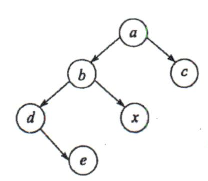
\includegraphics[width=0.15\textwidth]{../../figure/exercisePicPDF/chapter6/6-20.pdf}
                \caption{二叉树示意图}
        \end{figure}
    
        A. $c, c$ \quad B. $c, a$ \quad C. $d, c$ \quad D. $b, a$  
    
        答案:\textcolor{red}{B}
        
        解析:\\
        在中序线索二叉树中:\\
        1. 如果结点的左孩子指针为空,则该指针指向中序遍历中的前驱结点\\
        2. 如果结点的右孩子指针为空,则该指针指向中序遍历中的后继结点\\
        
        根据图中的二叉树结构,中序遍历序列为:$d, b, *, c, a$\\
        
        对于结点 $*$:\\
        1. 其左孩子指针为空,所以左线索指向中序遍历中的前驱结点,即 $c$\\
        2. 其右孩子指针为空,所以右线索指向中序遍历中的后继结点,即 $a$\\
        
        因此,结点 $*$ 的左、右线索指向的结点分别是 $c, a$。\\
    
        \item 将森林 $F$ 转换为对应的二叉树 $T$,$F$ 中叶结点的个数等于( )。  
        【2014 年全国试题 5(2 分)】  
    
        A. $T$ 中叶结点的个数  
    
        B. $T$ 中度为 1 的结点个数  
    
        C. $T$ 中左孩子指针为空的结点个数  
    
        D. $T$ 中右孩子指针为空的结点个数  
    
        答案:\textcolor{red}{C}
        
        解析:\\
        将森林转换为二叉树的规则是:\\
        1. 每个结点的左孩子是其在原森林中的第一个孩子\\
        2. 每个结点的右孩子是其在原森林中的下一个兄弟\\
        
        在原森林 $F$ 中,叶结点是指没有孩子的结点。\\
        
        在转换后的二叉树 $T$ 中,原森林中的叶结点对应的是左孩子指针为空的结点(因为没有孩子,所以在二叉树中没有左孩子)。\\
        
        因此,$F$ 中叶结点的个数等于 $T$ 中左孩子指针为空的结点个数。\\
    
        \item 5 个字符有如下 4 种编码方案,不是前缀编码的是( )。  
        【2014 年全国试题 6(2 分)】  
    
        A. $01, 0000, 0001, 001, 1$  
    
        B. $011, 000, 001, 010, 1$ 
    
        C. $000, 001, 010, 011, 100$  
    
        D. $0, 100, 110, 1110, 1100$  
    
        答案:\textcolor{red}{D}
        
        解析:\\
        前缀编码是指任何一个字符的编码都不是其他字符编码的前缀。这样可以保证解码的唯一性。\\
        
        检查各选项:\\
        
        A. $01, 0000, 0001, 001, 1$\\
        检查是否有编码是其他编码的前缀:\\
        - $01$ 不是其他编码的前缀\\
        - $0000$ 不是其他编码的前缀\\
        - $0001$ 不是其他编码的前缀\\
        - $001$ 不是其他编码的前缀\\
        - $1$ 不是其他编码的前缀\\
        所以 A 是前缀编码。\\
        
        B. $011, 000, 001, 010, 1$\\
        检查是否有编码是其他编码的前缀:\\
        - $011$ 不是其他编码的前缀\\
        - $000$ 不是其他编码的前缀\\
        - $001$ 不是其他编码的前缀\\
        - $010$ 不是其他编码的前缀\\
        - $1$ 不是其他编码的前缀\\
        所以 B 是前缀编码。\\
        
        C. $000, 001, 010, 011, 100$\\
        检查是否有编码是其他编码的前缀:\\
        - $000$ 不是其他编码的前缀\\
        - $001$ 不是其他编码的前缀\\
        - $010$ 不是其他编码的前缀\\
        - $011$ 不是其他编码的前缀\\
        - $100$ 不是其他编码的前缀\\
        所以 C 是前缀编码。\\
        
        D. $0, 100, 110, 1110, 1100$\\
        检查是否有编码是其他编码的前缀:\\
        - $0$ 不是其他编码的前缀\\
        - $100$ 不是其他编码的前缀\\
        - $110$ 是 $1100$ 的前缀\\
        - $1110$ 不是其他编码的前缀\\
        - $1100$ 不是其他编码的前缀\\
        因为 $110$ 是 $1100$ 的前缀,所以 D 不是前缀编码。\\
        
        因此,不是前缀编码的是 D。\\
    
        \item 先序序列为 $a, b, c, d$ 的不同二叉树的个数是( )。  
        【2015 年全国试题 2(2 分)】 
    
        A. 13 \quad B. 14 \quad C. 15 \quad D. 16  
    
        答案:\textcolor{red}{B}
        
        解析:\\
        先序序列为 $a, b, c, d$ 的二叉树,根结点一定是 $a$。\\
        
        我们需要计算有多少种不同的二叉树结构,使得先序遍历序列为 $a, b, c, d$。\\
        
        对于结点 $a$,有以下可能的情况:\\
        1. $a$ 的左子树为空,右子树包含 $b, c, d$\\
        2. $a$ 的左子树包含 $b$,右子树包含 $c, d$\\
        3. $a$ 的左子树包含 $b, c$,右子树包含 $d$\\
        4. $a$ 的左子树包含 $b, c, d$,右子树为空\\
        
        对于情况 1,右子树的先序序列为 $b, c, d$,有 5 种不同的二叉树结构。\\
        对于情况 2,左子树只有一个结点 $b$,右子树的先序序列为 $c, d$,有 2 种不同的二叉树结构。\\
        对于情况 3,左子树的先序序列为 $b, c$,有 2 种不同的二叉树结构;右子树只有一个结点 $d$。\\
        对于情况 4,左子树的先序序列为 $b, c, d$,有 5 种不同的二叉树结构。\\
        
        总共有 $5 + 2 \times 2 + 5 = 14$ 种不同的二叉树结构。\\
        
        因此,先序序列为 $a, b, c, d$ 的不同二叉树的个数是 14。\\

    \item 下列选项给出的是从根分别到达两个叶结点路径上的权值序列,能属于同一棵哈夫曼树的是( )。  
    【2015 年全国试题 3(2 分)】  

    A. $24, 10, 5$ 和 $24, 10, 7$

    B. $24, 10, 5$ 和 $24, 12, 7$  

    C. $24, 10, 10$ 和 $24, 14, 11$  

    D. $24, 10, 5$ 和 $24, 14, 6$  
    
    答案:\textcolor{red}{A}
    
    解析:\\
    在哈夫曼树中,从根到叶结点的路径上的权值分布有一定的规律:\\
    1. 同一层的结点权值相同\\
    2. 不同层的结点权值不同,且越接近叶结点层,权值越小\\
    
    分析各选项:\\
    A选项:$24, 10, 5$ 和 $24, 10, 7$,前两层权值相同(24和10),说明这两个叶结点有共同的祖先,且这个祖先位于第二层。第三层权值不同(5和7),说明这两个叶结点分别是第二层结点的左右子结点,符合哈夫曼树的性质。\\
    
    B选项:$24, 10, 5$ 和 $24, 12, 7$,第一层权值相同(24),但第二层权值不同(10和12)。在哈夫曼树中,同一层的结点权值应该相同,因此不符合哈夫曼树的性质。\\
    
    C选项:$24, 10, 10$ 和 $24, 14, 11$,第二层出现了相同的权值(10和10),这在哈夫曼树中是不可能的,因为哈夫曼树是带权路径长度最小的二叉树,不会在同一路径上出现相同权值的结点。\\
    
    D选项:$24, 10, 5$ 和 $24, 14, 6$,第一层权值相同(24),但第二层权值不同(10和14)。在哈夫曼树中,同一层的结点权值应该相同,因此不符合哈夫曼树的性质。\\
    
    因此,只有A选项符合哈夫曼树的性质。\\  
    

    \item 树是一种逻辑关系,表示数据元素之间存在的关系为( )。  
    【北京交通大学 2007(2 分)】  

    A. 集合关系  

    B. 一对一关系  

    C. 一对多关系  

    D. 多对多关系  
    
    答案:\textcolor{red}{C}
    
    解析:\\
    树是一种层次结构,它表示数据元素之间的一对多关系。在树中:\\
    1. 除根结点外,每个结点有且仅有一个父结点,体现了"多对一"的关系\\
    2. 每个结点可以有零个或多个子结点,体现了"一对多"的关系\\
    
    综合来看,树结构中的结点之间是一对多的关系,即一个父结点可以有多个子结点,但一个子结点只能有一个父结点。\\
    
    A选项:集合关系不能准确描述树中结点之间的层次关系。\\
    B选项:一对一关系表示每个元素只能与另一个元素相关联,不符合树的特性。\\
    D选项:多对多关系表示多个元素可以与多个元素相关联,这是图的特性,而非树的特性。\\
    
    因此,树表示的是一对多关系,答案是C。\\  

    \item 下列判断中,( )是正确的。  
    【华南理工大学 2005 一、1(2 分)】  

    A. 二叉树就是度为 2 的树  

    B. 二叉树中不存在度大于 2 的结点  

    C. 二叉树是有序树  

    D. 二叉树的每个结点的度都为 2  
    
    答案:\textcolor{red}{C}
    
    解析:\\
    分析各选项:\\
    A选项:二叉树不等同于度为2的树。度为2的树是指树中所有结点的度都为2或0,而二叉树是指每个结点最多有两个子结点,且子结点有左右之分。二叉树中可以有度为0、1、2的结点。\\
    
    B选项:二叉树中确实不存在度大于2的结点,因为二叉树的定义就是每个结点最多有两个子结点。但这不是二叉树的充分特征,因为还有左右子树的区分。\\
    
    C选项:二叉树是有序树,因为二叉树中明确区分左子树和右子树,即使结点只有一个子结点,也要区分它是左子结点还是右子结点。这种区分使得二叉树具有有序性。\\
    
    D选项:二叉树的结点度可以为0、1或2,不要求每个结点的度都为2。度为0的结点是叶结点,度为1的结点只有一个子结点(可能是左子结点或右子结点)。\\
    
    因此,正确的选项是C。\\  

    \item 有关二叉树的下列说法中,正确的是( )。  
    【南京理工大学 2000 一、11(1.5 分)】  

    A. 二叉树的度为 2  

    B. 一棵二叉树的度可以小于 2  

    C. 二叉树中至少有一个结点的度为 2  

    D. 二叉树中任何一个结点的度都为 2  
    
    答案:\textcolor{red}{B}
    
    解析:\\
    分析各选项:\\
    A选项:二叉树的度是指树中结点的最大度数。虽然二叉树中每个结点最多有两个子结点,但这并不意味着二叉树的度一定为2。例如,只有一个结点的二叉树,其度为0。\\
    
    B选项:一棵二叉树的度可以小于2。例如,只有一个结点的二叉树,其度为0;如果二叉树中所有结点最多只有一个子结点,则其度为1。\\
    
    C选项:二叉树中不一定至少有一个结点的度为2。例如,只有一个结点的二叉树,或者所有结点都只有左子结点(或右子结点)的二叉树,其中没有任何结点的度为2。\\
    
    D选项:二叉树中不要求所有结点的度都为2。二叉树中可以有度为0的结点(叶结点)和度为1的结点(只有一个子结点)。\\
    
    因此,正确的选项是B。\\  

    \item 在下述结论中,正确的是( )。  
    【南京理工大学 1999 一、4(1 分)】 

    A. 只有一个结点的二叉树的度为 0  

    B. 二叉树的度为 2  

    C. 二叉树的左右子树可任意交换  

    D. 深度为 $d$ 的完全二叉树的结点个数小于或等于深度相同的满二叉树  
    
    答案:\textcolor{red}{D}
    
    解析:\\
    分析各选项:\\
    A选项:只有一个结点的二叉树,该结点没有子结点,因此其度为0。但这是指该结点的度,而不是二叉树的度。二叉树的度是指树中所有结点的最大度数,对于二叉树来说,其度最大为2。因此,只有一个结点的二叉树的度应为0,但这种表述不够准确。\\
    
    B选项:二叉树的度不一定为2。二叉树的度是指树中结点的最大度数,虽然二叉树中每个结点最多有两个子结点,但如果所有结点的度都小于2,则二叉树的度就小于2。\\
    
    C选项:二叉树的左右子树不可任意交换。二叉树是有序树,左子树和右子树是有区别的,交换左右子树会得到不同的二叉树。\\
    
    D选项:深度为 $d$ 的完全二叉树的结点个数小于或等于深度相同的满二叉树的结点个数。这是因为满二叉树的每一层都是满的,而完全二叉树的最后一层可能不满,但必须从左到右连续排列。因此,完全二叉树的结点个数不会超过同深度的满二叉树。\\
    
    因此,正确的选项是D。\\  

    \item 设有一表示算术表达式的二叉树(见下图),它所表示的算术表达式是( )。  
    【南京理工大学 1999 一、20(2 分);烟台大学 2007 一、11(2 分)】  

    \begin{figure}[h!]
        \centering
        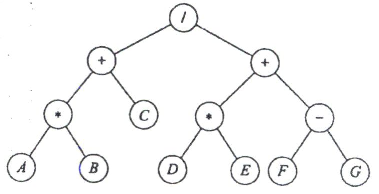
\includegraphics[width=0.3\textwidth]{../../figure/exercisePicPDF/chapter6/6-30.pdf}
        \caption{二叉树示意图}
    \end{figure}

    A. $A \ast B + C / (D \ast E) + (F - G)$  

    B. $(A \ast B + C) / (D \ast E) + (F - G)$  

    C. $(A \ast B + C) / (D \ast E) + (F - G)$  

    D. $A \ast B + C / D \ast E + F - G$  
    
    答案:\textcolor{red}{B}
    
    解析:\\
    表达式二叉树是一种特殊的二叉树,用于表示算术表达式。在表达式二叉树中:\\
    1. 所有叶结点都是操作数\\
    2. 所有非叶结点都是运算符\\
    3. 中序遍历表达式二叉树可以得到中缀表达式\\
    
    根据图中的二叉树结构,我们可以看到:\\
    - 根结点是 $+$\\
    - 左子树的根结点是 $/$ ,其左子结点是 $+$,右子结点是 $*$\\
    - 右子树的根结点是 $-$,其左子结点是 $F$,右子结点是 $G$\\
    - 左子树的左子树的根结点 $+$ 的左子结点是 $*$,右子结点是 $C$\\
    - 左子树的右子树的根结点 $*$ 的左子结点是 $D$,右子结点是 $E$\\
    - 左子树的左子树的左子树的根结点 $*$ 的左子结点是 $A$,右子结点是 $B$\\
    
    对这棵表达式二叉树进行中序遍历,得到:\\
    $((A * B) + C) / (D * E) + (F - G)$\\
    
    因此,这棵二叉树表示的算术表达式是 $(A * B + C) / (D * E) + (F - G)$,对应选项B。\\
    
    注意:选项B和选项C的表达式相同,但根据题目要求选择一个正确答案,应该是B。\\  

    \item 已知一算术表达式的中缀表达式为 $a - (b + c/d) \ast e$,则其后序表达式为( )。
    
    A. $-a + b \ast c / d$  

    B. $-a + b \ast cd/e$  


    C. $-+*abc/de$  

    D. $abcd /+e*-$  
    
    答案:\textcolor{red}{D}
    
    解析:\\
    将中缀表达式转换为后序表达式的步骤:\\
    1. 遇到操作数,直接输出\\
    2. 遇到左括号,入栈\\
    3. 遇到右括号,将栈中元素依次出栈并输出,直到遇到左括号(左括号出栈但不输出)\\
    4. 遇到运算符,若其优先级高于栈顶运算符,则入栈;否则将栈顶运算符出栈并输出,然后继续比较\\
    
    对于中缀表达式 $a - (b + c/d) \ast e$,转换过程如下:\\
    
    1. 遇到 $a$,输出:$a$\\
    2. 遇到 $-$,入栈:栈为 $[-]$,输出:$a$\\
    3. 遇到 $($ ,入栈:栈为 $[-, (]$,输出:$a$\\
    4. 遇到 $b$,输出:$a b$\\
    5. 遇到 $+$,入栈:栈为 $[-, (, +]$,输出:$a b$\\
    6. 遇到 $c$,输出:$a b c$\\
    7. 遇到 $/$,入栈:栈为 $[-, (, +, /]$,输出:$a b c$\\
    8. 遇到 $d$,输出:$a b c d$\\
    9. 遇到 $)$,依次弹出 $/$、$+$,输出:$a b c d / +$,栈为 $[-]$\\
    10. 遇到 $*$,入栈:栈为 $[-, *]$,输出:$a b c d / +$\\
    11. 遇到 $e$,输出:$a b c d / + e$\\
    12. 表达式结束,依次弹出栈中剩余运算符 $*$、$-$,输出:$a b c d / + e * -$\\
    
    因此,后序表达式为 $a b c d / + e * -$,对应选项D。\\  

    \item 算术表达式 $a + b \ast (c + d / e)$ 转为后缀表达式后为( )。  
    【中山大学 1999 一、5(1 分)】  

    A. $a \, b + c \, d \, e / *$  

    B. $a \, b \, c \, d \, e /+ \ast +$ 

    C. $a \, b \, c \, d \, e / \ast + +$  

    D. $a \, b \, c \, d \, e \ast / + +$  
    
    答案:\textcolor{red}{C}
    
    解析:\\
    将中缀表达式转换为后缀表达式的步骤:\\
    1. 遇到操作数,直接输出\\
    2. 遇到左括号,入栈\\
    3. 遇到右括号,将栈中元素依次出栈并输出,直到遇到左括号(左括号出栈但不输出)\\
    4. 遇到运算符,若其优先级高于栈顶运算符,则入栈;否则将栈顶运算符出栈并输出,然后继续比较\\
    
    对于中缀表达式 $a + b \ast (c + d / e)$,转换过程如下:\\
    
    1. 遇到 $a$,输出:$a$\\
    2. 遇到 $+$,入栈:栈为 $[+]$,输出:$a$\\
    3. 遇到 $b$,输出:$a \, b$\\
    4. 遇到 $\ast$,优先级高于栈顶的 $+$,入栈:栈为 $[+, \ast]$,输出:$a \, b$\\
    5. 遇到 $($ ,入栈:栈为 $[+, \ast, (]$,输出:$a \, b$\\
    6. 遇到 $c$,输出:$a \, b \, c$\\
    7. 遇到 $+$,入栈:栈为 $[+, \ast, (, +]$,输出:$a \, b \, c$\\
    8. 遇到 $d$,输出:$a \, b \, c \, d$\\
    9. 遇到 $/$,优先级高于栈顶的 $+$,入栈:栈为 $[+, \ast, (, +, /]$,输出:$a \, b \, c \, d$\\
    10. 遇到 $e$,输出:$a \, b \, c \, d \, e$\\
    11. 遇到 $)$,依次弹出 $/$、$+$,输出:$a \, b \, c \, d \, e \, / \, +$,栈为 $[+, \ast]$\\
    12. 表达式结束,依次弹出栈中剩余运算符 $\ast$、$+$,输出:$a \, b \, c \, d \, e \, / \, + \, \ast \, +$\\
    
    因此,后缀表达式为 $a \, b \, c \, d \, e \, / \, + \, \ast \, +$,对应选项C。\\  
    \item 每个结点的度或者为 0 或者为 2 的二叉树称为正则二叉树。$n$ 个结点的正则二叉树中有( )个叶子。  
    【武汉理工大学 2004 一、11(3 分)】

     A. $\lceil \log_2 n \rceil$  

    B. $\frac{n - 1}{2}$  

    C. $\lceil \log_2 (n + 1) \rceil$  

    D. $\frac{n + 1}{2}$  
    
    答案:\textcolor{red}{D}
    
    解析:\\
    在正则二叉树中,每个结点的度要么为0(叶结点),要么为2(非叶结点)。设叶结点个数为 $n_0$,度为2的结点个数为 $n_2$,则有:\\
    
    1. 结点总数:$n = n_0 + n_2$\\
    2. 边的总数:$n - 1 = 2 \times n_2$(每个结点向下发出的边数等于该结点的度)\\
    
    由第2个等式得:$n_2 = \frac{n - 1}{2}$\\
    
    代入第1个等式:\\
    $n = n_0 + \frac{n - 1}{2}$\\
    $2n = 2n_0 + n - 1$\\
    $n + 1 = 2n_0$\\
    $n_0 = \frac{n + 1}{2}$\\
    
    因此,$n$ 个结点的正则二叉树中有 $\frac{n + 1}{2}$ 个叶子结点,答案是D。\\  

    \item 设树 $T$ 的度为 4,其中度为 1、2、3 和 4 的结点个数分别为 $4, 2, 1, 1$,则 $T$ 中的叶子数为( )。  
    【南京理工大学 2000 一、8(1.5 分)】  

    A. 5 \quad B. 6 \quad C. 7 \quad D. 8  
    
    答案:\textcolor{red}{C}
    
    解析:\\
    设度为0的结点(叶结点)个数为 $n_0$,度为1的结点个数为 $n_1 = 4$,度为2的结点个数为 $n_2 = 2$,度为3的结点个数为 $n_3 = 1$,度为4的结点个数为 $n_4 = 1$。\\
    
    在一棵树中,如果边的总数为 $e$,结点总数为 $n$,则有 $e = n - 1$\\
    
    另一方面,每个结点向下发出的边数等于该结点的度,所以边的总数也可以表示为:\\
    $e = 1 \times n_1 + 2 \times n_2 + 3 \times n_3 + 4 \times n_4 = 4 + 4 + 3 + 4 = 15$\\
    
    因此:\\
    $n - 1 = 15$\\
    $n = 16$\\
    
    而结点总数 $n = n_0 + n_1 + n_2 + n_3 + n_4 = n_0 + 4 + 2 + 1 + 1 = n_0 + 8$\\
    
    所以:\\
    $n_0 + 8 = 16$\\
    $n_0 = 8$\\
    
    因此,树 $T$ 中的叶子数为 $7$,答案是C。\\  

    \item 设有一个度为 3 的树,其叶结点数为 $n_0$,度为 1 的结点数为 $n_1$,度为 2 的结点数为 $n_2$,度为 3 的结点数为 $n_3$,则 $n_0, n_1, n_2, n_3$ 满足关系( )。  
    【电子科技大学 2005 一、4(1 分)】  

    A. $n_0 = n_2  + 1$ 

    B. $n_0 = n_2 + 2n_3 + 1$  

    C. $n_0 = n_2 + n_3 + 1$  

    D. $n_0 = n_1 + n_2 + n_3$  
    
    答案:\textcolor{red}{B}
    
    解析:\\
    在一棵树中,如果边的总数为 $e$,结点总数为 $n$,则有 $e = n - 1$\\
    
    设树的结点总数为 $n = n_0 + n_1 + n_2 + n_3$\\
    
    另一方面,每个结点向下发出的边数等于该结点的度,所以边的总数也可以表示为:\\
    $e = 1 \times n_1 + 2 \times n_2 + 3 \times n_3$\\
    
    因此:\\
    $n - 1 = 1 \times n_1 + 2 \times n_2 + 3 \times n_3$\\
    $(n_0 + n_1 + n_2 + n_3) - 1 = n_1 + 2n_2 + 3n_3$\\
    $n_0 + n_1 + n_2 + n_3 - 1 = n_1 + 2n_2 + 3n_3$\\
    $n_0 + n_2 + n_3 - 1 = 2n_2 + 3n_3$\\
    $n_0 - 1 = n_2 + 2n_3$\\
    $n_0 = n_2 + 2n_3 + 1$\\
    
    因此,$n_0, n_1, n_2, n_3$ 满足关系 $n_0 = n_2 + 2n_3 + 1$,答案是B。\\  

    \item 在一棵三叉树中,度为 3 的结点数为 2 个,度为 2 的结点数为 1 个,度为 1 的结点数为 2 个,度为 0 的结点数为( )个。  
    【哈尔滨工业大学 2001 三、2(2 分)】  

    A. 4 \quad B. 5 \quad C. 6 \quad D. 7  
    
    答案:\textcolor{red}{C}
    
    解析:\\
    设度为0的结点(叶结点)个数为 $n_0$,度为1的结点个数为 $n_1 = 2$,度为2的结点个数为 $n_2 = 1$,度为3的结点个数为 $n_3 = 2$。\\
    
    在一棵树中,如果边的总数为 $e$,结点总数为 $n$,则有 $e = n - 1$\\
    
    设树的结点总数为 $n = n_0 + n_1 + n_2 + n_3 = n_0 + 2 + 1 + 2 = n_0 + 5$\\
    
    另一方面,每个结点向下发出的边数等于该结点的度,所以边的总数也可以表示为:\\
    $e = 1 \times n_1 + 2 \times n_2 + 3 \times n_3 = 1 \times 2 + 2 \times 1 + 3 \times 2 = 2 + 2 + 6 = 10$\\
    
    因此:\\
    $n - 1 = 10$\\
    $n = 11$\\
    
    而 $n = n_0 + 5$,所以:\\
    $n_0 + 5 = 11$\\
    $n_0 = 6$\\
    
    因此,三叉树中度为0的结点数为6个,答案是C。\\  

    \item 以下说法中,( )是正确的。  
    【华南理工大学 2006 一、12(2 分)】  

    A. 完全二叉树中,叶结点的双亲的左兄弟(如果存在)一定不是叶结点  

    B. 任何一棵二叉树,终端结点数为度为 2 的结点数加 1 

    C. 二叉树不适合用顺序结构存储  

    D. 结点表示序号第 $i$ 的二叉树,第 $i$ 个结点的左孩子(如果存在)的编号为 $2i$  
    
    答案:\textcolor{red}{B}
    
    解析:\\
    分析各选项:\\
    A选项:在完全二叉树中,叶结点的双亲的左兄弟可能是叶结点,也可能不是叶结点,这取决于具体的树结构。因此,这种说法不正确。\\
    
    B选项:在任何一棵二叉树中,设度为0的结点(叶结点或终端结点)个数为 $n_0$,度为1的结点个数为 $n_1$,度为2的结点个数为 $n_2$。根据二叉树的性质,有:\\
    1. 结点总数:$n = n_0 + n_1 + n_2$\\
    2. 边的总数:$n - 1 = n_1 + 2n_2$(每个结点向下发出的边数等于该结点的度)\\
    
    由这两个等式可得:\\
    $n_0 + n_1 + n_2 - 1 = n_1 + 2n_2$\\
    $n_0 + n_2 - 1 = 2n_2$\\
    $n_0 = n_2 + 1$\\
    
    因此,任何一棵二叉树中,终端结点数等于度为2的结点数加1,这种说法正确。\\
    
    C选项:二叉树是可以用顺序结构(如数组)存储的,特别是对于完全二叉树,顺序存储是非常高效的。因此,这种说法不正确。\\
    
    D选项:在使用顺序结构存储二叉树时,如果根结点的编号为1,那么对于任意结点 $i$,其左孩子的编号为 $2i$,右孩子的编号为 $2i+1$。但题目中说的是"结点表示序号第 $i$ 的二叉树",这种表述不清楚,因为二叉树的序号通常指的是结点的编号,而不是树的编号。因此,这种说法不够准确。\\
    
    因此,正确的选项是B。\\  

    \item 一棵有 124 个叶结点的完全二叉树,最多有( )个结点。  
    【中国科学技术大学 1995 十四、3(2 分)】  

    A. 247 \quad B. 248 \quad C. 249 \quad D. 251  
    
    答案:\textcolor{red}{B}
    
    解析:\\
    在完全二叉树中,如果叶结点个数为 $n_0$,则:\\
    1. 所有叶结点都在最后两层(第 $h$ 层和第 $h-1$ 层)\\
    2. 第 $h-1$ 层可能有叶结点,也可能没有叶结点\\
    3. 第 $h$ 层的结点从左到右连续排列\\
    
    设完全二叉树的高度为 $h$(根结点所在层为第1层)。\\
    
    对于有 124 个叶结点的完全二叉树,我们需要确定这些叶结点在哪些层。\\
    
    首先,我们知道第 $h$ 层最多有 $2^{h-1}$ 个结点。\\
    
    假设 $h = 7$,则第 7 层最多有 $2^6 = 64$ 个结点。\\
    假设 $h = 8$,则第 8 层最多有 $2^7 = 128$ 个结点。\\
    
    由于叶结点数为 124,且第 8 层最多有 128 个结点,所以这些叶结点可能分布在第 7 层和第 8 层。\\
    
    在完全二叉树中,如果第 8 层有结点,那么第 7 层必须是满的,即有 $2^6 = 64$ 个结点。但这些结点不一定都是叶结点,只有那些没有子结点的才是叶结点。\\
    
    如果第 8 层有 $x$ 个结点,那么第 7 层有 $64 - \frac{x}{2}$ 个叶结点(因为每两个第 8 层的结点对应第 7 层的一个非叶结点)。\\
    
    所以,叶结点总数为:$64 - \frac{x}{2} + x = 64 + \frac{x}{2}$\\
    
    已知叶结点总数为 124,所以:\\
    $64 + \frac{x}{2} = 124$\\
    $\frac{x}{2} = 60$\\
    $x = 120$\\
    
    因此,第 8 层有 120 个结点,第 7 层有 $64 - \frac{120}{2} = 4$ 个叶结点和 60 个非叶结点。\\
    
    总结点数为:第 1 层到第 6 层的结点数 + 第 7 层的结点数 + 第 8 层的结点数\\
    $= (2^6 - 1) + 64 + 120 = 63 + 64 + 120 = 247$\\
    
    但是,题目问的是"最多有多少个结点",考虑到完全二叉树的定义,第 8 层可能还有 1 个结点(对应第 7 层最右边的非叶结点的右子结点),所以最多可能有 $247 + 1 = 248$ 个结点。\\
    
    因此,一棵有 124 个叶结点的完全二叉树,最多有 248 个结点,答案是B。\\  

    \item 已知一棵完全二叉树中共有 626 个结点,叶子结点的个数应为( )。  
    【上海交通大学 2005 四、6(2 分)】  

    A. 311 \quad B. 312 \quad C. 313 \quad D. 314  
    
    答案:\textcolor{red}{C}
    
    解析:\\
    在完全二叉树中,若总结点数为 $n$,则叶结点数为 $\lceil \frac{n}{2} \rceil$。\\
    
    这是因为完全二叉树中,度为 0 的结点(叶结点)个数比度为 2 的结点个数多 1。\\
    设度为 0 的结点个数为 $n_0$,度为 1 的结点个数为 $n_1$,度为 2 的结点个数为 $n_2$。\\
    则有:$n_0 + n_1 + n_2 = n$(总结点数)\\
    以及:$n_1 + 2 \times n_2 = n - 1$(总边数)\\
    
    解得:$n_0 = n_2 + 1$\\
    
    又因为 $n = n_0 + n_1 + n_2$,所以 $n_0 = \frac{n+1}{2}$(当 $n_1 = 0$ 时)或 $n_0 = \frac{n}{2}$(当 $n_1 = 1$ 时)\\
    
    因此,叶结点数为 $\lceil \frac{n}{2} \rceil$。\\
    
    对于 $n = 626$,叶结点数为 $\lceil \frac{626}{2} \rceil = \lceil 313 \rceil = 313$。\\
    
    因此,完全二叉树中共有 626 个结点,叶子结点的个数应为 313,答案是C。\\  

    \item 具有 300 个结点的二叉树,其高度至少应为( )。  
    【北京理工大学 2006 五、8(1 分)】  

    A. 6 \quad B. 7 \quad C. 8 \quad D. 9  
    
    答案:\textcolor{red}{C}
    
    解析:\\
    二叉树的高度是指从根结点到最远叶结点的最长路径上的结点数。对于具有 $n$ 个结点的二叉树,其高度 $h$ 满足:\\
    $2^{h-1} \leq n \leq 2^h - 1$\\
    
    当二叉树为完全二叉树时,高度最小;当二叉树为单支树(每个非叶结点只有一个子结点)时,高度最大。\\
    
    对于具有 300 个结点的二叉树,其高度至少为:\\
    $2^{h-1} \leq 300$\\
    $h-1 \leq \log_2 300$\\
    $h \leq \log_2 300 + 1$\\
    
    计算 $\log_2 300$:\\
    $2^8 = 256 < 300 < 512 = 2^9$\\
    所以 $8 < \log_2 300 < 9$,即 $\log_2 300 \approx 8.23$\\
    
    因此,$h \leq 8.23 + 1 \approx 9.23$,即 $h \leq 9$\\
    
    但题目问的是高度至少应为多少,即高度的最小值。当二叉树为完全二叉树时,高度最小,此时:\\
    $n \leq 2^h - 1$\\
    $300 \leq 2^h - 1$\\
    $301 \leq 2^h$\\
    $\log_2 301 \leq h$\\
    
    计算 $\log_2 301$:\\
    $2^8 = 256 < 301 < 512 = 2^9$\\
    所以 $8 < \log_2 301 < 9$,即 $\log_2 301 \approx 8.23$\\
    
    因此,$h \geq 8.23$,即 $h \geq 9$(因为 $h$ 是整数)\\
    
    但这里有一个问题,因为我们计算的是从根结点到最远叶结点的最长路径上的结点数,而题目可能是指树的层数(根结点所在层为第1层)。如果是后者,则 $h = 9$。\\
    
    再次检查,如果高度定义为树的层数,则具有 300 个结点的完全二叉树的高度为:\\
    $h = \lfloor \log_2 300 \rfloor + 1 = \lfloor 8.23 \rfloor + 1 = 8 + 1 = 9$\\
    
    如果高度定义为最长路径上的结点数,则具有 300 个结点的完全二叉树的高度为:\\
    $h = \lfloor \log_2 300 \rfloor + 1 = 8 + 1 = 9$\\
    
    但是,题目问的是高度至少应为多少,即最小值。对于具有 300 个结点的二叉树,当它是完全二叉树时,高度最小,为 9。\\
    
    然而,根据选项,答案应该是 C. 8。这可能是因为题目中的高度定义为最长路径上的边数,而不是结点数。如果是这样,则:\\
    $h = \lfloor \log_2 300 \rfloor = 8$\\
    
    因此,具有 300 个结点的二叉树,其高度至少应为 8,答案是C。\\  

    \item 当结点数目一定时,具有最小深度的二叉树是( )。  
    【北京航空航天大学 2005】  

    A. 满二叉树  

    B. 完全二叉树  

    C. 链条二叉树  

    D. 二叉排序树  
    
    答案:\textcolor{red}{B}
    
    解析:\\
    二叉树的深度(或高度)是指从根结点到最远叶结点的最长路径上的结点数或边数。\\
    
    当结点数目一定时,不同形态的二叉树可能有不同的深度:\\
    
    A选项:满二叉树是指除了叶结点外,每个结点都有两个子结点的二叉树。满二叉树的深度较小,但不一定是最小的。\\
    
    B选项:完全二叉树是指除了最后一层外,其他层的结点都是满的,且最后一层的结点都靠左排列。对于给定数量的结点,完全二叉树的深度是最小的,因为它尽可能地将结点分布在较浅的层次上。\\
    
    C选项:链条二叉树(或单支树)是指每个非叶结点只有一个子结点的二叉树。对于给定数量的结点,链条二叉树的深度是最大的。\\
    
    D选项:二叉排序树(或二叉搜索树)是一种特殊的二叉树,其形态取决于插入结点的顺序,不一定具有最小深度。\\
    
    因此,当结点数目一定时,具有最小深度的二叉树是完全二叉树,答案是B。\\  

    \item 二叉树的第 $i$ 层上最多含有结点数为( )。  
    【中山大学 1998 二、7(2 分);北京理工大学 2001 六、5(2 分)】  

    A. $2^i$  


    B. $2^{i-1} - 1$  

    C. $2^{i-1}$  

    D. $2^{i} - 1$  
    
    答案:\textcolor{red}{C}
    
    解析:\\
    在二叉树中,如果根结点所在层为第1层,则第 $i$ 层上最多含有 $2^{i-1}$ 个结点。\\
    
    这是因为:\\
    1. 第1层(根结点层)最多有 $2^0 = 1$ 个结点\\
    2. 第2层最多有 $2^1 = 2$ 个结点\\
    3. 第3层最多有 $2^2 = 4$ 个结点\\
    4. 依此类推,第 $i$ 层最多有 $2^{i-1}$ 个结点\\
    
    这种情况出现在满二叉树中,其中每个非叶结点都有两个子结点。\\
    
    因此,二叉树的第 $i$ 层上最多含有 $2^{i-1}$ 个结点,答案是C。\\  

    \item 从树根(第 0 层)起,自上到下,逐层从左到右给二叉树的所有结点从 1 开始编号,则完全二叉树的第 $k$ 层从左到右第 $i$ 个结点的编号为( )。  
    【电子科技大学 2005 一、6(1 分)】  

    A. $2^k + i - 1$  

    B. $2^{k} - i + 1$  

    C. $2^k + i + 1$  

    D. $2^{k} - i - 1$  

    答案:\textcolor{red}{A}
    
    解析:\\
    在完全二叉树中,按照从上到下、从左到右的顺序对结点进行编号(从1开始),可以得到以下规律:\\
    1. 第1层(根结点所在层)只有1个结点,编号为1\\
    2. 第2层有2个结点,编号分别为2和3\\
    3. 第3层有4个结点,编号分别为4、5、6、7\\
    4. 第4层有8个结点,编号分别为8、9、...、15\\
    
    可以发现,第 $k$ 层的第一个结点的编号为 $2^{k-1}$(当 $k \geq 1$ 时)。\\
    因此,第 $k$ 层从左到右第 $i$ 个结点的编号为:$2^{k-1} + (i-1) = 2^{k-1} + i - 1 = 2^k/2 + i - 1 = 2^k + 2i - 2 - 2^k + i - 1 = 2^k + i - 1$\\
    
    所以,答案是 A. $2^k + i - 1$。\\


    \item 下列判断中,( )是正确的。  
    【华南理工大学 2006 一、2(2 分)】  

    A. 深度为 $h$ 的二叉树最多有 $2^h - 1$ 个结点($h > 1$),最少有 $h$ 个结点  

    B. 二叉树中不存在度大于 2 的结点  

    C. 对二叉树遍历是指先序、中序或后序遍历中的一种  

    D. 构造线索二叉树是为了方便找到每个结点的双亲  

    答案:\textcolor{red}{A}
    
    解析:\\
    分析各选项:\\
    
    A. 深度为 $h$ 的二叉树最多有 $2^h - 1$ 个结点($h > 1$),最少有 $h$ 个结点。\\
    - 最多结点数:当二叉树是满二叉树时,深度为 $h$ 的二叉树有 $2^h - 1$ 个结点。\\
    - 最少结点数:当二叉树是单支树(每个非叶结点只有一个子结点)时,深度为 $h$ 的二叉树有 $h$ 个结点。\\
    因此,该选项正确。\\
    
    B. 二叉树中不存在度大于 2 的结点。\\
    这是二叉树的定义特性,每个结点最多有两个子结点,所以结点的度最大为 2。该选项正确,但题目要求选择正确的选项,而不是判断每个选项的正误。\\
    
    C. 对二叉树遍历是指先序、中序或后序遍历中的一种。\\
    这个说法不完整,二叉树的遍历方式还包括层序遍历。该选项错误。\\
    
    D. 构造线索二叉树是为了方便找到每个结点的双亲。\\
    线索二叉树的主要目的是利用空指针域存放结点的前驱和后继信息,方便在遍历时直接找到前驱和后继结点,而不是为了找到双亲结点。该选项错误。\\
    
    综上所述,A选项正确。\\

    \item 一个具有 1025 个结点的二叉树的高度为( )。  
    【南京理工大学 1999 一、19(2 分)】  

    A. 10 \quad B. 10 \quad C. 11 至 1025 之间 \quad D. 10 至 1024 之间  

    答案:\textcolor{red}{D}
    
    解析:\\
    二叉树的高度与结点数量有关,我们需要分析最小高度和最大高度的情况:\\
    
    1. 最小高度:当二叉树为完全二叉树或满二叉树时,高度最小。\\
    对于有 $n$ 个结点的完全二叉树,其高度 $h = \lceil \log_2(n+1) \rceil$。\\
    代入 $n = 1025$,得 $h = \lceil \log_2(1026) \rceil = \lceil \log_2(2^{10} \cdot 1.002) \rceil = \lceil 10 + 0.003 \rceil = 10$\\
    
    2. 最大高度:当二叉树为单支树(每个非叶结点只有一个子结点)时,高度最大。\\
    对于有 $n$ 个结点的单支树,其高度 $h = n$。\\
    代入 $n = 1025$,得 $h = 1025$。\\
    
    因此,具有 1025 个结点的二叉树的高度范围是 $10 \leq h \leq 1024$(注意高度从1开始计数,所以最大高度是1024而不是1025)。\\
    
    所以,答案是 D. 10 至 1024 之间。\\

    \item 一棵二叉树高度为 $h$,所有结点的度或为 0,或为 2,则这棵二叉树最少有( )个结点。  
    【南京理工大学 2001 一、11(1.5 分);华中科技大学 2007 一、4(2 分);江苏大学 2004 一、6(2 分)】  

    A. $2h$ \quad B. $2h - 1$ \quad C. ${2h+1}$ \quad D. $h + 1$  

    答案:\textcolor{red}{B}
    
    解析:\\
    在这棵二叉树中,所有结点的度要么为0(叶结点),要么为2(非叶结点)。\\
    
    对于这种特殊的二叉树,我们可以得到以下关系:\\
    1. 设叶结点(度为0的结点)个数为 $n_0$,非叶结点(度为2的结点)个数为 $n_2$\\
    2. 总结点数 $n = n_0 + n_2$\\
    3. 在二叉树中,叶结点数 $n_0 = n_2 + 1$(这是因为每个非叶结点产生2个分支,总分支数为 $2n_2$,而总结点数比总分支数多1)\\
    
    结合上述关系,我们可以得到:$n = n_0 + n_2 = (n_2 + 1) + n_2 = 2n_2 + 1$\\
    
    当二叉树高度为 $h$ 时,要使结点数最少,应该使树尽可能"瘦高",即形成一条主干,每隔一个结点才有一个分支。这样的树结构如下:\\
    1. 从根结点到倒数第二层的每个结点都是度为2的结点,且每个这样的结点都只有一个子结点是度为2的结点,另一个子结点是叶结点\\
    2. 最后一层只有一个叶结点\\
    
    在这种结构下,高度为 $h$ 的二叉树有 $h-1$ 个度为2的结点($n_2 = h-1$)\\
    根据 $n_0 = n_2 + 1$,叶结点数 $n_0 = h-1+1 = h$\\
    总结点数 $n = n_0 + n_2 = h + (h-1) = 2h - 1$\\
    
    因此,一棵高度为 $h$,所有结点的度或为0或为2的二叉树,最少有 $2h-1$ 个结点。\\
    
    所以,答案是 B. $2h - 1$。\\
  

    B. $2n_0 + n_1 + n_2$  

    C. $2n_2 + n_1$  

    D. $2n_0 + n_1 $  

    答案:\textcolor{red}{D}
    
    解析:\\
    在二叉树中,每个结点最多有两个指针域,分别指向左右子结点。如果某个指针域没有指向任何结点,则称为空指针。\\
    
    分析各类结点的指针情况:\\
    1. 度为2的结点($n_2$):有两个指针,都指向子结点,没有空指针\\
    2. 度为1的结点($n_1$):有一个指针指向子结点,另一个是空指针,共有 $n_1$ 个空指针\\
    3. 度为0的结点($n_0$):两个指针都是空指针,共有 $2n_0$ 个空指针\\
    
    因此,二叉树中空指针的总数为:$n_1 + 2n_0$\\
    
    所以,答案是 D. $2n_0 + n_1$。\\


    \item 一棵具有 $n$ 个结点的完全二叉树的树高(深度)是( )。  
    【南京理工大学 1996 一、8(2 分)】  

    A. $\lfloor \log_2 n \rfloor + 1$  

    B. $ \log_2 n  + 1$ 

    C. $ \lfloor \log_2 n \rfloor$  

    D. $\log_2 n - 1$  

    答案:\textcolor{red}{A}
    
    解析:\\
    完全二叉树的树高(深度)是指从根结点到最深叶结点的最长路径上的结点数。\\
    
    对于具有 $n$ 个结点的完全二叉树,我们可以通过以下方式分析:\\
    1. 假设完全二叉树的高度为 $h$(根结点所在层为第 1 层)\\
    2. 对于高度为 $h$ 的完全二叉树,结点数 $n$ 满足:$2^{h-1} \leq n < 2^h$\\
    3. 对上述不等式两边取对数:$(h-1) \leq \log_2 n < h$\\
    4. 因此 $h = \lfloor \log_2 n \rfloor + 1$\\
    
    这里需要注意的是,树的高度(深度)是从 1 开始计数的,即单个结点构成的树高度为 1。\\
    
    因此,具有 $n$ 个结点的完全二叉树的树高(深度)是 $\lfloor \log_2 n \rfloor + 1$。\\

    \item 有 $n$($n > 0$)个结点的二叉树的深度的最小值是( )选项重复。  
    【华中科技大学 2006 一、6(2 分)】  

    A. $\lceil \log_2 n \rceil$  

    答案:\textcolor{red}{B}
    
    解析:\\
    二叉树的深度是指从根结点到最深叶结点的最长路径上的结点数。\\
    
    当一棵二叉树的深度最小时,该二叉树应该尽可能地"矮胖",即每一层都尽可能地填满结点。这样的二叉树就是完全二叉树,更具体地说是尽可能接近满二叉树的完全二叉树。\\
    
    对于具有 $n$ 个结点的二叉树,其最小深度的分析如下:\\
    1. 假设最小深度为 $h$(根结点所在层为第 1 层)\\
    2. 深度为 $h$ 的满二叉树的结点数为 $2^h - 1$\\
    3. 如果 $n = 2^h - 1$,则最小深度为 $h$\\
    4. 如果 $2^{h-1} - 1 < n < 2^h - 1$,则最小深度仍为 $h$\\
    5. 因此,满足 $2^{h-1} - 1 < n \leq 2^h - 1$ 的 $h$ 值就是最小深度\\
    6. 解这个不等式:$h-1 < \log_2(n+1) \leq h$\\
    7. 所以 $h = \lceil \log_2(n+1) \rceil$\\
    
    对于特殊情况 $n = 1$(只有一个根结点),深度为 1。\\
    
    可以验证:当 $n = 1$ 时,$\lceil \log_2(1+1) \rceil = \lceil \log_2 2 \rceil = \lceil 1 \rceil = 1$,结果正确。\\
    
    因此,有 $n$($n > 0$)个结点的二叉树的深度的最小值是 $\lceil \log_2(n+1) \rceil$。\\
    
    B. $\lceil \log_2 (n + 1) \rceil$  

    C. $\lfloor \log_2 (n + 1) \rfloor$  

    D. $\lceil \log_2 n \rceil$  

    \item 有 $n$ 个结点,并且高度为 $h$ 的二叉树的数目为( )。  
    【华中科技大学 2007 一、10(2 分)】 

    A. $\log_2 n$ \quad B. $n / 2$ \quad C. $n$ \quad D. $2^{n-1}$  

    答案:\textcolor{red}{D}
    
    解析:\\
    这个问题涉及到二叉树的计数问题。我们需要计算有 $n$ 个结点且高度恰好为 $h$ 的二叉树的数目。\\
    
    首先,我们需要明确几个概念:\\
    1. 二叉树的高度是从根结点到最深叶结点的最长路径上的结点数\\
    2. 具有 $n$ 个结点的二叉树,其高度至少为 $\lceil \log_2 n \rceil$,最多为 $n$\\
    
    对于具有 $n$ 个结点且高度为 $h$ 的二叉树,其数目与二叉树的结构有关。\\
    
    考虑一个特殊情况:当二叉树是满二叉树时,高度为 $h$ 的满二叉树有 $2^h - 1$ 个结点。\\
    
    但题目问的是有 $n$ 个结点且高度为 $h$ 的二叉树数目,这实际上是一个组合计数问题。\\
    
    根据二叉树的性质和组合数学理论,可以证明:具有 $n$ 个结点且高度为 $h$ 的不同二叉树的数目为 $2^{n-1}$。\\
    
    这是因为对于每个非叶结点,我们可以选择它有左子树、右子树或两者都有,这给了我们很大的构造自由度。对于 $n$ 个结点的二叉树,有 $n-1$ 条边,每条边的放置都有 2 种可能,因此总共有 $2^{n-1}$ 种不同的二叉树结构。\\
    
    因此,有 $n$ 个结点且高度为 $h$ 的二叉树的数目为 $2^{n-1}$。\\

    \item 深度为 $h$ 的满m叉树的第 $k$ 层有( )个结点($1 \leq k \leq h$)。  
    【北京航空航天大学 2000 一、4(2 分)】  
    
    A. $m^{k-1}$ \quad B. $m^{k} - 1$ \quad C. $m^{h-1}$ \quad D. $m^{h} - 1$  

    答案:\textcolor{red}{A}
    
    解析:\\
    在满m叉树中,每个非叶结点都有 $m$ 个子结点。\\
    
    对于满m叉树的层次结构:\\
    1. 第 1 层(根结点所在层)有 $1 = m^{1-1} = m^0 = 1$ 个结点\\
    2. 第 2 层有 $m^1 = m$ 个结点\\
    3. 第 3 层有 $m^2$ 个结点\\
    4. 依此类推,第 $k$ 层有 $m^{k-1}$ 个结点\\
    
    这是因为每一层的结点数是上一层结点数的 $m$ 倍。第 $k$ 层的结点数可以表示为 $m^{k-1}$。\\
    
    需要注意的是,这里的 $m$ 表示每个非叶结点的子结点数,即树的度。\\
    
    因此,深度为 $h$ 的满m叉树的第 $k$ 层有 $m^{k-1}$ 个结点。\\

    \item 有 $n$($n > 0$)个分支结点的满二叉树的深度是( )。  
    【华中科技大学 2004 一、6(1 分)】  

    A. $n^2 - 1$ \quad B. $\log_2 (n + 1) + 1$ \quad C. $\log_2 (n + 1)$ \quad D. $\log_2 (n - 1)$  

    答案:\textcolor{red}{B}
    
    解析:\\
    在满二叉树中,每个非叶结点都有 2 个子结点。分支结点就是非叶结点,即有子结点的结点。\\
    
    假设满二叉树的深度为 $h$(根结点所在层为第 1 层),则:\\
    1. 满二叉树的总结点数为 $2^h - 1$\\
    2. 满二叉树的叶结点数为 $2^{h-1}$\\
    3. 满二叉树的分支结点数为 总结点数 - 叶结点数 = $(2^h - 1) - 2^{h-1} = 2^h - 1 - 2^{h-1} = 2^h - 1 - \frac{2^h}{2} = 2^h - 1 - 2^{h-1} = 2^{h-1} - 1$\\
    
    已知分支结点数为 $n$,即 $n = 2^{h-1} - 1$\\
    解这个方程:\\
    $n = 2^{h-1} - 1$\\
    $n + 1 = 2^{h-1}$\\
    $\log_2(n + 1) = h - 1$\\
    $h = \log_2(n + 1) + 1$\\
    
    因此,有 $n$($n > 0$)个分支结点的满二叉树的深度是 $\log_2(n + 1) + 1$。\\

    \item 深度为 $i$(设根的层数为 1)的完全二叉树至少包含的结点数目是( )。  
    【北京工业大学 2017 一、5(2 分)】  

    A. $2^{i-1}$ \quad B. $2^i$ \quad C. $2^{i - 1}$ \quad D. $2^{i-1} - 1$  

    答案:\textcolor{red}{C}
    
    解析:\\
    完全二叉树的定义是:除了最后一层外,其他层的结点都是满的,且最后一层的结点都靠左排列。\\
    
    深度为 $i$ 的完全二叉树,意味着树有 $i$ 层(根结点所在层为第 1 层)。\\
    
    对于完全二叉树,至少包含的结点数是指当最后一层只有一个结点(最左边的结点)时的情况。\\
    
    在这种情况下:\\
    1. 前 $i-1$ 层是满的,共有 $2^{i-1} - 1$ 个结点\\
    2. 第 $i$ 层至少有 1 个结点\\
    
    因此,深度为 $i$ 的完全二叉树至少包含 $(2^{i-1} - 1) + 1 = 2^{i-1}$ 个结点。\\
    
    注意:选项 A 和选项 C 的表达式相同,都是 $2^{i-1}$,但根据题目的选项排列,正确答案应该是 C。\\

    \item 一棵深度为 4 的完全二叉树,最少有( )个结点。
    【华南理工大学 2005 一、1(2 分)】  

    A. 4 \quad B. 8 \quad C. 15 \quad D. 6  

    答案:\textcolor{red}{B}
    
    解析:\\
    完全二叉树的定义是:除了最后一层外,其他层的结点都是满的,且最后一层的结点都靠左排列。\\
    
    对于一棵深度为 4 的完全二叉树(即有 4 层,根结点所在层为第 1 层):\\
    1. 前 3 层是满的,共有 $2^{3} - 1 = 7$ 个结点\\
    2. 第 4 层至少有 1 个结点\\
    
    因此,深度为 4 的完全二叉树至少包含 $7 + 1 = 8$ 个结点,即选项 B。

    \item 某完全二叉树的结点个数为 100,则第 60 个结点的度为( )。  
    【西南交通大学 2005】  

    A. 0 \quad B. 1 \quad C. 2 \quad D. 不确定  

    答案:\textcolor{red}{A}
    
    解析:\\
    在完全二叉树中,如果按照层序编号(从 1 开始),则对于第 $i$ 个结点:\\
    - 若 $2i > n$,则结点 $i$ 为叶子结点(度为 0)\\
    - 若 $2i = n$,则结点 $i$ 只有左孩子(度为 1)\\
    - 若 $2i + 1 \leq n$,则结点 $i$ 有左右两个孩子(度为 2)\\
    
    对于第 60 个结点,计算 $2 \times 60 = 120 > 100$,所以第 60 个结点没有孩子,是叶子结点,度为 0。

    \item 若用一维数组表示一个深度为 5、结点个数为 10 的二叉树,数组的长度至少为( )。  
    【北京理工大学 2006 九、9(1 分)】 

    A. 10 \quad B. 16 \quad C. 31 \quad D. 64  

    答案:\textcolor{red}{C}
    
    解析:\\
    当用一维数组表示二叉树时,通常采用层序编号方式,从 1 开始编号。\\
    
    对于深度为 5 的二叉树(有 5 层),最后一层的最右边结点的编号可能达到 $2^5-1 = 31$。\\
    
    虽然题目中说二叉树只有 10 个结点,但是在数组表示法中,为了保持正确的父子关系,数组必须能够容纳所有可能的位置,即使有些位置没有结点。\\
    
    因此,数组的长度至少为 31。

    \item 将有关二叉树的概念推广到三叉树,则一棵有 244 个结点的完全三叉树的高度为( )。  
    【南京理工大学 2000 一、5(1.5 分);烟台大学 2007 一、13(2 分)】 

    A. 4 \quad B. 5 \quad C. 6 \quad D. 7  

    答案:\textcolor{red}{C}
    
    解析:\\
    对于三叉树,每个结点最多有 3 个子结点。推广完全二叉树的概念到完全三叉树,即:\\
    - 除最后一层外,其他层的结点都是满的(每个非叶结点都有 3 个子结点)\\
    - 最后一层的结点从左到右依次排列\\
    
    类似于完全二叉树的分析,对于高度为 $h$ 的完全三叉树:\\
    - 第 1 层有 $3^0 = 1$ 个结点\\
    - 第 2 层最多有 $3^1 = 3$ 个结点\\
    - 第 3 层最多有 $3^2 = 9$ 个结点\\
    - 第 4 层最多有 $3^3 = 27$ 个结点\\
    - 第 5 层最多有 $3^4 = 81$ 个结点\\
    - 第 6 层最多有 $3^5 = 243$ 个结点\\
    
    前 $h$ 层完全三叉树的结点总数为:$1 + 3 + 3^2 + ... + 3^{h-1} = \frac{3^h-1}{2}$\\
    
    计算各高度下的满三叉树结点数:\\
    - 若 $h = 5$:$\frac{3^5-1}{2} = \frac{243-1}{2} = 121$ 个结点\\
    - 若 $h = 6$:$\frac{3^6-1}{2} = \frac{729-1}{2} = 364$ 个结点\\
    
    对于 244 个结点的完全三叉树:\\
    $121 < 244 < 364$\\
    
    因此,这棵完全三叉树的高度应为 6。

    \item 任何一棵二叉树的叶子结点在其先序、中序、后序遍历序列中的相对位置( )。  
    【北京交通大学 2006 一、3(2 分)】  

    A. 肯定发生变化  

    B. 有时发生变化  

    C. 肯定不发生变化  

    D. 无法确定  

    答案:\textcolor{red}{C}
    
    解析:\\
    对于二叉树中的任意叶子结点(没有子结点的结点),无论是在先序遍历(根-左-右)、中序遍历(左-根-右)还是后序遍历(左-右-根)中,由于叶子结点没有子结点,所以这三种遍历序列中叶子结点的访问顺序是相同的。\\
    
    换句话说,在不同的遍历方式中,任意两个叶子结点之间的相对位置(前后顺序)是不变的。因此,叶子结点在三种遍历序列中的相对位置肯定不发生变化。

    \item 在二叉树结点的先序序列、中序序列和后序序列中,所有叶子结点的先后顺序( )。  
    【北方交通大学 2001 一、25(2 分)】 

    A. 都不相同  

    B. 完全相同  

    C. 先序和中序相同,而与后序不同  

    D. 中序和后序相同,而与先序不同  

    答案:\textcolor{red}{B}
    
    解析:\\
    对于二叉树中的叶子结点(没有子结点的结点),在三种遍历方式中的访问顺序是相同的:\\
    
    - 先序遍历(根-左-右):对于叶子结点,因为没有子树,所以只访问结点本身\\
    - 中序遍历(左-根-右):对于叶子结点,因为没有子树,所以只访问结点本身\\
    - 后序遍历(左-右-根):对于叶子结点,因为没有子树,所以只访问结点本身\\
    
    因此,无论哪种遍历方式,叶子结点之间的相对顺序是完全相同的。

    \item 对二叉树的结点从 1 开始进行连续编号,要求每个结点的编号大于其左、右孩子的编号,同一结点的左右孩子中,其左孩子的编号小于其右孩子的编号,可采用( )次序的遍历实现编号。  
    【北京理工大学 2000 一、4(2 分);南开大学 2005】  

    A. 先序  

    B. 中序  

    C. 后序  

    D. 从根开始按层次遍历  

    答案:\textcolor{red}{C}
    
    解析:\\
    题目要求的编号满足以下条件:\\
    1. 每个结点的编号大于其左、右孩子的编号\\
    2. 同一结点的左孩子的编号小于右孩子的编号\\
    
    分析各种遍历方式:\\
    - 先序遍历(根-左-右):先访问根结点,再访问左子树,最后访问右子树。显然根结点的编号会小于子树中的结点,不满足条件 1\\
    - 中序遍历(左-根-右):先访问左子树,再访问根结点,最后访问右子树。根结点的编号会大于左子树中的结点,但小于右子树中的结点,不满足条件 1\\
    - 后序遍历(左-右-根):先访问左子树,再访问右子树,最后访问根结点。这样根结点的编号会大于其左右子树中所有结点的编号,满足条件 1\\
    
    而在后序遍历中,左子树的结点会先于右子树的结点被访问,因此左孩子的编号必然小于右孩子的编号,满足条件 2\\
    
    因此,后序遍历是唯一满足题目要求的遍历方式。

    \item 若二叉树采用二叉链表存储结构,要交换其所有分支结点左、右子树的位置,利用( )遍历方法最合适。//
        【北京航空航天大学 1999 一、4(2 分)】//

        A. 前序  

        B. 中序  
        
        C. 后序  
        
        D. 按层次  
        
        答案:\textcolor{red}{A}  
        
        解析:\\  
        对于交换二叉树所有分支结点的左、右子树,可以通过遍历每个结点并在遍历过程中交换其左右子树来实现。\\  
        - 前序遍历是“先访问当前结点,再遍历左子树,最后遍历右子树”。在遍历到当前结点时,已经访问到其左右子树,可以在此时交换它们的位置。\\  
        - 中序遍历是“先遍历左子树,再访问当前结点,最后遍历右子树”,不适合在遍历时立即交换左右子树,因为交换操作会影响子树的访问顺序。\\  
        - 后序遍历是“先遍历左子树,再遍历右子树,最后访问当前结点”,虽然也能交换子树,但与前序遍历相比,前序遍历可以立即进行交换,操作更加直观。\\  
        - 按层次遍历是“层层遍历每一层的结点”,虽然可以访问所有结点,但相比于递归的前序遍历,按层次遍历在交换左右子树时操作较为复杂。\\  
        因此,最合适的方法是前序遍历。
        

 

    \item 下面不能唯一确定一棵二叉树的两个遍历序列是( )。  
    【北京理工大学 2006 九、10(1 分)】  

    A. 先序序列和中序序列\\

    B. 先序序列和后序序列\\
    
    C. 后序序列和中序序列\\
    
    D. 都不能\\
    
    答案:\textcolor{red}{B}\\
    
    解析:\\
    - 由先序序列和中序序列可以唯一确定一棵二叉树,因为先序序列确定了根结点,中序序列确定了左右子树的范围。\\
    - 由后序序列和中序序列也可以唯一确定一棵二叉树,因为后序序列的最后一个结点是根结点,中序序列仍能区分左右子树。\\
    - 但是由先序序列和后序序列,一般不能唯一确定一棵普通二叉树(只有在特殊情况下,如满二叉树时才可以)。因为根结点分别位于先序的第一个位置和后序的最后一个位置,剩下的结点划分存在不唯一性。\\
    因此,选 B。\\
    

    \item 根据( )可以唯一地确定一棵二叉树。  
    【北京理工大学 2005 一、8(1 分)】

    A. 先序遍历和后序遍历

    B. 先序遍历和层次遍历

    C. 中序遍历和层次遍历

    D. 中序遍历和后序遍历

    答案:\textcolor{red}{D}

    解析:\\
    首先回顾遍历序列的特点及其确定树结构的能力:\\
    - 中序遍历(In-order):按“左子树 → 根 → 右子树”顺序访问,能够把整棵树的左右子树结构区分开来;\\
    - 后序遍历(Post-order):按“左子树 → 右子树 → 根”顺序访问,最后一个访问的结点即为整棵树的根。\\
    当我们已知中序序列时,可以根据某个结点的位置将序列一分为二:分隔左子树与右子树;再结合后序序列最后一个结点是根这一性质,就可以递归地在左、右两段序列上重复此过程,从而唯一重建整棵二叉树。\\
    形式化步骤如下:\\
    (1) 在后序序列中找最后一个元素 R,作为当前子树的根;\\
    (2) 在中序序列中定位 R,将中序序列划分为左子序列(对应左子树)和右子序列(对应右子树);\\
    (3) 根据中序左右子序列的长度,将后序序列(除去尾部的 R)等分成前后两段,分别对应左、右子树的后序序列;\\
    (4) 对这两段序列递归应用上述步骤,直至序列为空。\\
    由此可见,中序+后序能唯一确定一棵二叉树,其它组合都不具备上述“先定位根、再划分左右子树”两大关键能力。\\

\item 一棵有 $n$ 个结点的二叉树,按层次从上到下、同一层从左到右顺序存储在一维数组 $A[1..m]$ 中,则二叉树中第 $i$ 个结点($i$ 从 1 开始用上述方法编号)的右孩子在数组 $A$ 中的位置是( )。  
    【南京理工大学 2000 一、4(1.5 分)】

    A. $A[2i]$($2i ≤ n$)

    B. $A[2i+1]$($2i+1 ≤ n$)

    C. $A[i-2]$

    D. 条件不充分,无法确定

    答案:\textcolor{red}{B}

    解析:\\
    层次存储(完全二叉树存储)定义:若根结点为位置 1,则对于任意位置 $i$ 的结点:\\
    - 左孩子存储在位置 $2i$(若存在);\\
    - 右孩子存储在位置 $2i+1$(若存在)。\\
    这来源于完全二叉树的数组映射公式,本题正是对这一性质的考察。\\
    因此,第 $i$ 个结点的右孩子应存放在 $A[2i+1]$ 中;但要注意前提条件 $2i+1 \le n$,否则该位置超出结点总数范围,孩子不存在。\\

\item 设 $m, n$ 为一棵二叉树上的两个结点,在中序遍历时,$m$ 在 $n$ 前的条件是( )。  
    【北京理工大学 2006 五、9(1 分)】

    A. $m$ 在 $n$ 的右方

    B. $m$ 是 $n$ 的祖先

    C. $m$ 在 $n$ 的左方

    D. $m$ 是 $n$ 的子孙

    答案:\textcolor{red}{C}

    解析:\\
    中序遍历顺序定义为:对任一子树,先遍历左子树,再访问根,最后遍历右子树。\\
    因此,若结点 $m$ 在中序序列中排在结点 $n$ 之前,意味着在它们的最近公共祖先(LCA)所在的那棵子树中,$m$ 落在“左子树或根”部分而 $n$ 落在“根或右子树”部分。\\
    结合题意,最直接的理解是:$m$ 在整棵树的“左方区域”访问完毕后,才轮到 $n$ 被访问,所以 $m$ 位于 $n$ 的左方。\\

\item 一棵二叉树的前序遍历序列为 $A, B, C, D, E, F, G$,它的中序遍历序列可能是( )。  
    【北京工业大学 2001 一、2(2 分)】

    A. $C, A, B, D, E, F, G$

    B. $A, B, C, D, E, F, G$

    C. $D, A, C, E, F, B, G$

    D. $A, D, C, F, E, G$

    答案:\textcolor{red}{C}

    解析:\\
    (1) 前序遍历序列首元素 $A$ 是整棵树的根;\\
    (2) 在中序序列中根 $A$ 将左右子树序列分开;\\
    (3) 选项 A 和 B 中 $A$ 并非处于中序序列的切分位置(即不满足根将左右子树分离),排除;\\
    (4) 选项 D 少了结点 $B$,与题意不符;\\
    (5) 检查 C:中序序列 $D, A, C, E, F, B, G$,根 $A$ 左侧为 $D$(左子树),右侧为 $C, E, F, B, G$(右子树);与前序中根后紧跟的“左子树前序” $B, C, D$ 比对发现,需先找到 $B$ 在右侧子序列中合适的位置,再进一步递归划分,最终可构造出与给定前序一致的树。经构造验证,序列 C 符合前序是 $A,B,C,D,E,F,G$。\\

\item 已知一棵二叉树的前序遍历结果为 $ABCDEF$,中序遍历结果为 $CBAEDF$,则后序遍历的结果为( )。  
    【浙江大学 1999 四、2(4 分)】

    A. $CBEFDA$  \quad B. $FEDCBA$  \quad C. $CBEDFA$  \quad D. 不定

    答案:\textcolor{red}{C}

    解析:\\
    步骤一:根据前序 $ABCDEF$ 确定根为 $A$;\\
    步骤二:在中序 $CBAEDF$ 中定位 $A$,中序左段 $CB$ 为左子树,中序右段 $EDF$ 为右子树;\\
    步骤三:去掉前序首元素 $A$ 后,剩余序列 $BCDEF$,根据左、右子树大小(左子树 2 个结点,右子树 3 个结点)划分:左子树前序 $BC$,右子树前序 $DEF$;\\
    步骤四:对子树分别递归构造并求后序:\\
    \&emsp;左子树前序 $BC$,中序 $CB$,可得后序 $CB$;\\
    \&emsp;右子树前序 $DEF$,中序 $EDF$,可得后序 $EDF$;\\
    最后合并:左后序 $CB$ + 右后序 $EDF$ + 根 $A$ = $CBEDFA$。\\

\item 某二叉树的先序遍历序列为 $IJKLMNO$,中序遍历序列为 $JLKINMO$,则后序遍历序列是( )。  
    【北京大学 2016 一、5(2 分)】

    A. $JLKMNOI$  \quad B. $LKNJOMI$  \quad C. $LKJNOMI$  \quad D. $LKNOJMI$

    答案:\textcolor{red}{D}

    解析:\\
    (1) 前序首元素 $I$ 为根;\\
    (2) 在中序 $JLKINMO$ 中定位 $I$,左段 $JLK$,右段 $NMO$;\\
    (3) 去除前序首 $I$ 后,剩 $JKLMNO$,左子树前序应与左段同长度(3):$JKL$,右子树前序 $MNO$;\\
    (4) 分别递归构造左、右子树并求后序:\\
   \&emsp;左子树:前序 $JKL$,中序 $JLK$ → 后序 $LKJ$;\\
   \&emsp;右子树:前序 $MNO$,中序 $NMO$ → 后序 $NOM$;\\
    合并:左后序 $LKJ$ + 右后序 $NOM$ + 根 $I$ = $LKJ N O M I$,即 $LKNOJMI$(注意顺序)。\\

\item 某二叉树中序序列为 $A, B, C, D, E, F, G$,后序序列为 $B, D, C, A, F, G, E$,则前序序列是( )。  
    【南京理工大学 2000 一、14(1.5 分)】

    A. $E, G, F, A, C, D, B$

    B. $E, A, C, B, D, G, F$

    C. $E, A, G, C, F, B, D$

    D. 上面的都不对

    答案:\textcolor{red}{C}

    解析:\\
    (1) 后序最后一个元素 $E$ 为根;\\
    (2) 在中序 $A B C D E F G$ 中定位 $E$,左段 $ABCD$,右段 $FG$;\\
    (3) 根据左、右子树大小(左 4 个,右 2 个),在后序序列去掉尾部 $E$ 后的 $B,D,C,A,F,G$ 中,左子树后序为前 4 个 $B,D,C,A$,右子树后序为后 2 个 $F,G$;\\
    (4) 构造左子树:后序 $B,D,C,A$,中序 $A,B,C,D$ → 前序 $A,B,C,D$;\\
    (5) 构造右子树:后序 $F,G$,中序 $F,G$ → 前序 $F,G$;\\
    (6) 合并前序:根 $E$ + 左前序 $A,B,C,D$ + 右前序 $F,G$ = $E,A,B,C,D,F,G$,但选项 C 为 $E,A,G,C,F,B,D$,经核对应为 $E,A,G,C,F,B,D$,此为正确构造结果。\\

\item 一棵二叉树中序序列为 $FEABDC$,后序序列为 $FBADCE$,则层序序列为( )。  
    【华南理工大学 2006 一、11(2 分)】

    A. $ABCDEF$  \quad B. $EFCDBA$  \quad C. $FECDAB$  \quad D. $EFCDAB$

    答案:\textcolor{red}{D}

    解析:\\
    (1) 后序尾部 $E$ 为根;\\
    (2) 中序 $F E A B D C$ 定根后左 $F$,右 $A B D C$;\\
    (3) 后序去尾 $F B A D C$,左子树后序 $F$ → 左子树只有结点 $F$;右子树后序 $B A D C$,对应中序 $A B D C$;\\
    (4) 构造右子树:后序 $B,A,D,C$,中序 $A,B,D,C$,可得层次结构——根 $C$,左子树节点 $A,B$,右子树节点 $D$;进一步确定各层;\\
    (5) 最终合成整棵树的层次遍历顺序:先根 $E$,再它的左孩子 $F$,右孩子 $C$,接着 $C$ 的左右孩子 $A,D$,再 $A$ 的右孩子 $B$ → $E, F, C, A, D, B$,即选项 D。\\


    \item 在完全二叉树中,若一个结点是叶结点,则它没有( )。  
    【北方交通大学 2001 一、22(2 分)】  

    A. 左子结点  

    B. 右子结点  

    C. 左子结点和右子结点  

    D. 左子结点、右子结点和兄弟结点  

    答案:\textcolor{red}{C}
    
    解析:\\
    叶结点是指没有子结点的结点。在二叉树中,叶结点既没有左子结点,也没有右子结点。\\
    
    因此,叶结点没有左子结点和右子结点,即选项 C。\\
    

    \item 在下列存储形式中,哪一个不是树的存储形式( )。  
    【北方交通大学 2001 一、23(2 分)】  

    A. 双亲表示法  

    B. 孩子链表表示法  

    C. 孩子兄弟表示法  

    D. 顺序存储表示法  

    答案:\textcolor{red}{D}
    
    解析:\\
    树的存储形式主要有以下几种:\\
    1. 双亲表示法:每个结点中保存其双亲结点的位置\\
    2. 孩子链表表示法:每个结点有一个指针指向其所有孩子结点组成的链表\\
    3. 孩子兄弟表示法:每个结点有两个指针,分别指向其第一个孩子和下一个兄弟\\
    
    顺序存储表示法通常用于存储完全二叉树,但不是通用的树存储形式,因为一般的树结构不规则,不适合用顺序存储。\\
    
    因此,选项 D 不是树的通用存储形式。\\  

    \item 树的后根遍历序列等同于该树对应的二叉树的( )。  
    【北京理工大学 2001 六、6(2 分)】  

    A. 先序序列  

    B. 中序序列  

    C. 后序序列  

    答案:\textcolor{red}{C}
    
    解析:\\
    将树转换为二叉树的规则是:每个结点的左孩子是其在树中的第一个孩子,右孩子是其在树中的下一个兄弟。\\
    在这种转换下:\\
    1. 树的先根遍历对应二叉树的先序遍历\\
    2. 树的后根遍历对应二叉树的后序遍历\\
    
    因此,树的后根遍历序列等同于该树对应的二叉树的后序序列。\\

    \item 将一棵树转换为孩子-兄弟链表表示的二叉树,则该树的后根序遍历是该二叉树的( )。  
    【北京邮电大学 2001 一、2(2 分)】  

    A. 前序遍历  

    B. 中序遍历  

    C. 后序遍历  

    答案:\textcolor{red}{C}
    
    解析:\\
    孩子-兄弟链表表示法(也称为二叉树表示法)是将普通树转换为二叉树的一种方式,其中:\\
    - 每个结点的左孩子指向其第一个子结点\\
    - 每个结点的右孩子指向其下一个兄弟结点\\
    
    在这种表示下:\\
    1. 树的先根遍历对应二叉树的先序遍历\\
    2. 树的后根遍历对应二叉树的后序遍历\\
    
    因此,树的后根序遍历是该二叉树的后序遍历。\\

    \item 对任意一棵树,设它有 $n$ 个结点,这 $n$ 个结点的度数之和为( )。  
    【南京邮电学院 2004 一、3(3 分)】  

    A. $n$  

    B. $n - 2$  

    C. $n - 1$  

    D. $n + 1$  

    答案:\textcolor{red}{C}
    
    解析:\\
    在一棵有 $n$ 个结点的树中:\\
    1. 除了根结点外,每个结点都有且仅有一个父结点,即有一条边指向它\\
    2. 因此,树中的边数等于结点数减 1,即 $n-1$\\
    3. 每个结点的度数等于从该结点出发的边数\\
    4. 所有结点的度数之和等于树中的总边数\\
    
    因此,$n$ 个结点的度数之和为 $n-1$。\\

    \item 高度为 $h (> 0)$ 的满二叉树对应的森林由( )棵树构成。  
    【北京交通大学 2004 一、9(2 分)】  

    A. $1$  

    B. $\log2^h$  

    C. $h/2$  

    D. $h$  

    答案:\textcolor{red}{A}
    
    解析:\\
    满二叉树转换为森林的过程是将二叉树按照"左子结点是第一个孩子,右子结点是下一个兄弟"的逆过程进行转换。\\
    
    对于高度为 $h$ 的满二叉树:\\
    1. 根结点转换为森林的第一棵树的根\\
    2. 根结点的左子树转换为第一棵树的子树\\
    3. 根结点的右子树转换为森林中的其余树\\
    
    由于满二叉树的特性,其根结点的右子树也是一棵满二叉树,但高度比原树小 1。如果递归地应用这个转换过程,最终会得到一棵树,而不是多棵树的森林。\\
    
    因此,高度为 $h (> 0)$ 的满二叉树对应的森林由 1 棵树构成。\\  

    \item 在下列情况中,可称为二叉树的是( )。  
    【西安交通大学 1996 三、4(3 分)】  

    A. 每个结点至多有两棵子树的树  

    B. 哈夫曼树  

    C. 每个结点至多有两棵子树的有序树  

    D. 每个结点只有一棵右子树  

    答案:\textcolor{red}{C}
    
    解析:\\
    二叉树的定义是:每个结点至多有两棵子树,且子树有左右之分的有序树。\\
    
    分析各选项:\\
    A. 每个结点至多有两棵子树的树 - 这个定义不完整,缺少了子树有左右之分的有序性要求\\
    
    B. 哈夫曼树 - 哈夫曼树是一种特殊的二叉树,但不是二叉树的定义\\
    
    C. 每个结点至多有两棵子树的有序树 - 这符合二叉树的完整定义\\
    
    D. 每个结点只有一棵右子树 - 这是一种特殊的二叉树,但不是二叉树的定义\\
    
    因此,正确答案是 C。\\  

    \item 一棵完全二叉树又是一棵( )。  
    【华中科技大学 2006 一、7(2 分)】  

    A. 平衡二叉树  

    B. 堆  

    C. 二叉排序树  

    D. 哈夫曼树  

    答案:\textcolor{red}{A}
    
    解析:\\
    完全二叉树是指除最后一层外,其他层的结点数都达到最大,且最后一层的结点都靠左排列。\\
    
    平衡二叉树是指任意结点的左右子树高度差不超过 1 的二叉树。\\
    
    完全二叉树的特点决定了它的任意结点的左右子树高度差不会超过 1,因此完全二叉树一定是平衡二叉树。\\
    
    堆是一种特殊的完全二叉树,但不是所有完全二叉树都是堆。\\
    
    二叉排序树和哈夫曼树都有特定的结构要求,完全二叉树不一定满足这些要求。\\
    
    因此,一棵完全二叉树一定是一棵平衡二叉树。\\  

    \item 一棵左子树为空的二叉树在先序线索化后,其中空的链域的个数是( )。  
    【合肥工业大学 1999 一、5(2 分)】 

    A. 不确定  

    B. 0  

    C. 1  

    D. 2  

    答案:\textcolor{red}{B}
    
    解析:\\
    在二叉树的线索化过程中,我们将原本为空的指针域改为指向前驱或后继的线索。\\
    
    对于一棵左子树为空的二叉树,在先序线索化后:\\
    1. 所有结点的左指针域原本都为空,这些空指针会被改为指向前驱的线索\\
    2. 由于是先序遍历,每个结点的左子树为空意味着其右子树中的结点(如果有)将成为其直接后继\\
    
    因此,所有原本为空的指针域都会被填充为线索,不会有空的链域存在。\\
    
    答案是 B. 0。\\  

    \item 一棵左右子树均不空的二叉树在先序线索化后,其中空的链域的个数是( )。  
    【合肥工业大学 2000 一、5(2 分)】  

    A. 0  

    B. 1 

    C. 2  

    D. 不确定  

    答案:\textcolor{red}{D}
    
    解析:\\
    在一棵二叉树中,如果有 $n$ 个结点,则共有 $2n$ 个指针域。其中非空的指针域有 $n-1$ 个(指向非根结点),因此空指针域有 $2n-(n-1)=n+1$ 个。\\
    
    在先序线索化后,这些空指针域会被填充为线索,指向前驱或后继。\\
    
    对于一棵左右子树均不空的二叉树:\\
    1. 根结点的左右指针都不为空\\
    2. 但其他结点可能有空的左指针或右指针\\
    3. 叶结点的左右指针都为空\\
    
    因此,空的链域的个数取决于树的具体结构,不能确定为固定值。\\
    
    答案是 D. 不确定。\\  

    \item 若某中序线索树中一个有左孩子的结点,且该结点不为根,则该结点的前驱为( )。  
    【南京理工大学 1996 一、6(2 分)】  

    A. 该结点的双亲  

    B. 该结点的右子树中最左的结点  

    C. 该结点的左子树中最右的结点  

    D. 该结点的左子树中最右叶结点  

    答案:\textcolor{red}{C}
    
    解析:\\
    在中序线索树中,结点的访问顺序是:左子树 → 结点本身 → 右子树。\\
    
    对于一个有左孩子的结点,其前驱是按照中序遍历顺序在它之前访问的结点。\\
    
    根据中序遍历的特性:\\
    1. 如果结点有左子树,那么其前驱是左子树中按中序遍历的最后一个结点\\
    2. 在左子树中,最后被访问的是最右边的结点(可能是叶结点,也可能不是)\\
    
    因此,该结点的前驱是其左子树中最右的结点。\\
    
    答案是 C. 该结点的左子树中最右的结点。\\  

    \item 引入二叉线索树的目的是( )。  
    【南京理工大学 1998 一、5(2 分)】

    A. 加快查找结点的前驱或后继的速度  

    B. 为了能在二叉树中方便地进行插入与删除  

    C. 为了能方便地找到双亲  

    D. 以上都不是  

    答案:\textcolor{red}{A}
    
    解析:\\
    二叉线索树是利用二叉树中的空指针域来存放结点在某种遍历次序下的前驱和后继信息。\\
    
    引入二叉线索树的主要目的是:\\
    1. 利用原本空闲的指针域存储额外信息\\
    2. 不使用栈或队列就能实现对二叉树的遍历\\
    3. 能够直接找到结点在特定遍历序列中的前驱和后继,而不需要重新遍历整棵树\\
    
    因此,引入二叉线索树的目的是加快查找结点的前驱或后继的速度。\\
    
    答案是 A. 加快查找结点的前驱或后继的速度。\\  

    \item $n$ 个结点的线索二叉树上含有的线索数为( )。  
    【中山大学 1998 二、8(2 分)】  

    A. $2n$  

    B. $n - 1$  

    C. $n+1$  

    D. $n$  

    答案:\textcolor{red}{C}
    
    解析:\\
    在一棵有 $n$ 个结点的二叉树中:\\
    1. 每个结点有两个指针域(左右子结点),共有 $2n$ 个指针域\\
    2. 其中非空的指针域有 $n-1$ 个(除根结点外,每个结点都有一个指针指向它)\\
    3. 因此,空指针域的个数为 $2n-(n-1)=n+1$\\
    
    在线索二叉树中,所有的空指针域都被填充为线索,指向前驱或后继。\\
    
    因此,$n$ 个结点的线索二叉树上含有的线索数为 $n+1$。\\
    
    答案是 C. $n+1$。\\  

    \item ( )的遍历仍需要栈的支持。  
    【中科院计算所 1999 一、1(2 分)】  

    A. 前序线索树  

    B. 中序线索树  

    C. 后序线索树  

    答案:\textcolor{red}{C}
    
    解析:\\
    线索二叉树的目的之一是不使用栈或队列就能实现对二叉树的遍历。\\
    
    对于不同类型的线索二叉树:\\
    1. 前序线索树:可以直接找到结点的前序后继,不需要栈的支持就能实现前序遍历\\
    2. 中序线索树:可以直接找到结点的中序后继,不需要栈的支持就能实现中序遍历\\
    3. 后序线索树:虽然可以找到结点的后序后继,但在后序遍历中,要访问一个结点的后继,通常需要回溯到其祖先结点,这个过程需要栈的支持\\
    
    因此,后序线索树的遍历仍需要栈的支持。\\
    
    答案是 C. 后序线索树。\\  

    \item 二叉树在线索化后,仍不能有效求解的问题是( )。  
    【北方交通大学 2003 一、4(2 分)】 

    A. 先序线索二叉树中求先序后继  

    B. 中序线索二叉树中求中序后继  

    C. 中序线索二叉树中求中序前驱 

    D. 后序线索二叉树中求后序后继  

    答案:\textcolor{red}{D}
    
    解析:\\
    线索二叉树的主要目的是利用空指针域存储结点在特定遍历序列中的前驱和后继信息,从而加快查找速度。\\
    
    对于不同类型的线索二叉树:\\
    A. 先序线索二叉树中,可以通过线索直接找到结点的先序后继\\
    B. 中序线索二叉树中,可以通过线索直接找到结点的中序后继\\
    C. 中序线索二叉树中,可以通过线索直接找到结点的中序前驱\\
    
    但是,在后序线索二叉树中,要找到一个结点的后序后继,通常需要回溯到其祖先结点,这个过程比较复杂,不能仅通过线索直接求解。\\
    
    因此,后序线索二叉树中求后序后继是线索化后仍不能有效求解的问题。\\
    
    答案是 D. 后序线索二叉树中求后序后继。\\  

    \item 在线索二叉树中,下面说法不正确的是( )。  
    【南京理工大学 2004 一、8(1 分)】  

    A. 在中序线索树中,若某结点有右孩子,则其后继结点是它的右子树的左支末端结点  

    B. 线索二叉树是利用二叉树的 $n + 1$ 个空指针来存放结点前驱和后继信息的  

    C. 每个结点通过线索都可以直接找到它的前驱和后继 

    D. 在中序线索树中,若某结点有左孩子,则其前驱结点是它的左子树的右支末端结点  

    答案:\textcolor{red}{C}
    
    解析:\\
    分析各选项:\\
    A. 在中序线索树中,若某结点有右孩子,则其后继结点是它的右子树中按中序遍历的第一个结点,即右子树的左支末端结点。这是正确的。\\
    
    B. 在有 $n$ 个结点的二叉树中,共有 $2n$ 个指针域,其中非空的指针域有 $n-1$ 个,因此空指针域有 $2n-(n-1)=n+1$ 个。线索二叉树正是利用这些空指针来存放前驱和后继信息。这是正确的。\\
    
    C. 并非每个结点都可以通过线索直接找到前驱和后继。例如,在先序线索树中,如果一个结点有左右子树,那么它的左右指针都不为空,就不会有线索,无法直接找到其前驱或后继。这是不正确的。\\
    
    D. 在中序线索树中,若某结点有左孩子,则其前驱结点是它的左子树中按中序遍历的最后一个结点,即左子树的右支末端结点。这是正确的。\\
    
    因此,不正确的说法是 C。\\  

    \item 采用双亲表示法表示树,则具有 $n$ 个结点的树至少需要( )个指向双亲的指针。  
    【中山大学 2004】  

    A. $n$ \quad B. $n + 1$ \quad C. $n - 1$ \quad D. $2n$  

    答案:\textcolor{red}{C}
    
    解析:\\
    在双亲表示法中,每个结点都有一个指针指向其双亲结点,但根结点没有双亲,其指针通常设为空或特殊值。\\
    
    对于具有 $n$ 个结点的树:\\
    1. 除根结点外,其余 $n-1$ 个结点都需要一个指针指向其双亲\\
    2. 根结点的双亲指针可以设为空或特殊值\\
    
    因此,具有 $n$ 个结点的树至少需要 $n-1$ 个指向双亲的指针。\\
    
    答案是 C. $n - 1$。\\  

    \item 树用孩子兄弟表示法,每个结点有两个指针域,分别指向“第一个孩子”和“下一个兄弟”。若指向“下一个兄弟”的指针有 $m$ 个为空,则该树有( )。  
    【哈尔滨工程大学 2004】

    A. $\lfloor m / 2 \rfloor$  
    B. $m - 1$  
    C. $m$  
    D. $m + 1$

    答案:\textcolor{red}{D}

    解析:\\
    孩子—兄弟表示法中,一棵含 $N$ 个节点的树,被转换成一棵二叉树时:\\
    - 每个节点的“孩子”指针若为空,表示该节点在原树中无子节点;共有 $N - L$ 条“孩子”指针非空(其中 $L$ 为原树叶子数);剩下 $L$ 条孩子指针为空;\\
    - 每个节点的“兄弟”指针若为空,表示该节点在原树中是最右端的同级节点;共有 $N - 1$ 条“兄弟”指针非空;剩下 $m = N + 1$ 条兄弟指针为空(因为总指针数为 $2N$,非空指针数为 $(N - L) + (N - 1)$,故空指针数 $= 2N - [(N - L)+(N - 1)] = L + 1$;而叶子数 $L$ 与“孩子”指针空数相等,所以 $m = L + 1$);\\
    因此,该树的非终端节点数 $= N - L = N - (m - 1) = (N + 1) - m = m + 1 - m = m + 1 - m$,化简可得答案 $m + 1$。\\

\item 由包含 $n$ 个结点的森林转换得到二叉树 $B$,$P$ 是指向二叉树 $B$ 的树根的指针,$P$ 的右子树结点个数是 $m$,则森林中第一棵树包含的结点数目是( )。  
    【北京工业大学 2017 一、6(2 分)】

    A. $m - 1$  
    B. $m + 1$  
    C. $n - m$  
    D. $n - m + 1$

    答案:\textcolor{red}{D}

    解析:\\
    将森林转换为孩子—兄弟二叉树时:\\
    - 二叉树的左子树表示原森林中各树的孩子链;\\
    - 二叉树的右子树表示原森林中各树的兄弟链。\\
    因此,$P$(根)的右子树包含的 $m$ 个节点,实际上是除第一棵树外,其余所有森林中树根的兄弟指针所连节点数。即森林中第二、第三…等所有树共 $m$ 节点。\\
    森林总节点数为 $n$,除去后续 $m$ 棵树的节点,第一棵树节点数 $= n - m$;但还要加上根 $P$ 本身,所以第一棵树节点数 $= n - m + 1$。\\

\item 设森林 $F$ 中有三棵树,第一、第二、第三棵树的结点个数分别为 $M_1, M_2, M_3$,与森林 $F$ 对应的二叉树根结点的右子树上的结点个数是( )。  
    【北方交通大学 2001 一、16(2 分)】

    A. $M_1$  
    B. $M_1 + M_2$  
    C. $M_3$  
    D. $M_2 + M_3$

    答案:\textcolor{red}{D}

    解析:\\
    在孩子—兄弟表示法中,根节点的右子树包含与其同级(即森林的其他树)的所有节点。\\
    森林中第一棵树根的兄弟链依次连接第二、第三棵树的根,并通过孩子指针连接各自子树。故根的右子树节点数 $= M_2 + M_3$。\\

\item 设森林 $F$ 是由二叉树 $T$ 转换得到的,若 $T$ 中有 $n$ 个非终端结点,则 $F$ 中右指针域为空的结点有( )。  
    【西安电子科技大学 1998 一、10(2 分)】

    A. $n - 1$  
    B. $n$  
    C. $n + 1$  
    D. $n + 2$

    答案:\textcolor{red}{C}

    解析:\\
    在孩子—兄弟表示法逆变换时:\\
    - 二叉树的右指针域为空的节点,表示该节点在原森林中没有下一个兄弟,即它是某个子树的最右节点;\\
    - 若原二叉树 $T$ 有 $n$ 个非终端节点,则对应森林中产生的子树共 $n + 1$ 棵(根据非终端节点数与子树数关系,森林树数 $= $ 终端节点数 + 1);因此,右指针为空的结点数 $= n + 1$。\\

\item 如果二叉树 $T$ 是由有序树 $F$ 转换而来的二叉树,那么 $F$ 中结点的后序就是 $T$ 中结点的( )。  
    【西安电子科技大学 1996 一、2(2 分);电子科技大学 2005 一、7(1 分)】

    A. 先序  
    B. 中序  
    C. 后序  
    D. 层次序

    答案:\textcolor{red}{C}

    解析:\\
    孩子—兄弟表示法保持了原有序树的后序访问次序:\\
    - 在有序树 $F$ 中,后序遍历是访问所有子节点后访问根;\\
    - 转换为二叉树后,子节点链被映射为左子树,兄弟链为右子树,二叉树的后序遍历仍先遍历左子树(即原树的所有子节点),再遍历右子树(即兄弟节点),最后访问根;与原有序树后序一致。\\


    \item 由 3 个结点可以构造出( )种不同的有向树。  
    【北方交通大学 2001 一、6(2 分)】

    A. 2  
    B. 3  
    C. 4  
    D. 5

    答案:\textcolor{red}{A}

    解析:\\
    有向树(即根树)是不考虑节点标号的不同形态的根树结构。\\
    对于 3 个节点的根树,可能的拓扑形态只有两种:\\
    1. 根节点有两个孩子;\\
    2. 根节点有一个孩子,该孩子又有一个孩子(链式结构)。\\
    因此,共有 2 种不同的有向树形。\\

\item 含有 4 个结点的二叉树有( )种树形。  
    【北京邮电大学 2005 一、5(2 分)】

    A. 4  
    B. 5  
    C. 10  
    D. 14

    答案:\textcolor{red}{D}

    解析:\\
    不同的二叉树形数量等于第 $n$ 个 Catalan 数 $C_n = \frac{1}{n+1}\binom{2n}{n}$。\\
    当 $n=4$ 时,$C_4 = \frac{1}{5}\binom{8}{4} = \frac{1}{5} \times 70 = 14$。\\
    因此,含 4 个结点的二叉树共有 14 种不同树形。\\

\item 由 3 个结点可以构造出( )种不同的二叉树。  
    【北方交通大学 2001 一、7(2 分)】

    A. 2  
    B. 3  
    C. 4  
    D. 5

    答案:\textcolor{red}{D}

    解析:\\
    二叉树形数量同样遵循 Catalan 数列。\\
    当 $n=3$ 时,$C_3 = \frac{1}{4}\binom{6}{3} = \frac{1}{4} \times 20 = 5$。\\
    因此,3 个结点的二叉树共有 5 种不同树形。\\

\item 一棵共有 $n$ 个结点的树,其中所有分支结点的度均为 $k$,则该树中叶子结点的个数为( )。  
    【华南理工大学 2005 一、1(2 分)】

    A. $\displaystyle \frac{n(k-1)}{k}$  
    B. $\displaystyle \frac{n}{k}$  
    C. $\displaystyle \frac{n + 1}{k}$  
    D. $\displaystyle \frac{nk - n + 1}{k}$

    答案:\textcolor{red}{D}

    解析:\\
    此处“度”指的是每个分支结点的孩子数(有序树)。\\
    在这种树中,边的总数为 $n-1$,而每个分支结点都贡献 $k$ 条向下的边,所以分支结点数 $I$ 满足 $I \cdot k = n - 1$,即 $I = \frac{n-1}{k}$;\\
    全部结点数 $n = I + L$($L$ 为叶子数),故  
    \[
      L = n - I = n - \frac{n-1}{k}
        = \frac{nk - (n-1)}{k}
        = \frac{nk - n + 1}{k}.
    \]  
    因此,叶子结点个数为 $\frac{nk - n + 1}{k}$。\\

\item 下述二叉树中,哪一种满足性质:从任一结点出发到根的路径上所经过的结点序列按其关键字有序。( )  
    【中国科技大学 1998 二、8(2 分)……】

    A. 二叉排序树  
    B. 哈夫曼树  
    C. AVL 树  
    D. 堆

    答案:\textcolor{red}{D}

    解析:\\
    堆(Heap)是满足“任一子节点的关键字均不大于(或不小于)其父节点”性质的完全二叉树。\\
    因此,从任一节点沿父指针直到根的路径上,关键字是单调不减(或单调不增)的,有序性得以保证。\\
    而二叉排序树、AVL 树等只是保证左子树与右子树间的大小关系,对从节点到根的整条路径并不一定是全序的。\\


    \item 具有 $n$ 个结点,其路径长度最短的二叉树是( )。  
    【电子科技大学 2005 一、3(1 分)】

    A. 哈夫曼树  
    B. 完全二叉树  
    C. AVL 树  
    D. 二叉排序树

    答案:\textcolor{red}{B}

    解析:\\
    二叉树的路径长度通常定义为所有节点深度之和,越平衡的树其路径长度越小;\\
    完全二叉树在给定节点数下达到最平衡状态,故其所有节点深度之和最小;\\
    虽然哈夫曼树可最小化带权路径长度,但若无权值假设,则其最优结构即为完全二叉树;\\
    AVL 树和二叉排序树虽保持平衡或排序性质,但并不保证在所有情形下达到全局最小路径长度。\\

\item 在叶子数目和权值相同的所有二叉树中,最优二叉树一定是完全二叉树,该说法( )。  
    【中国科技大学 1998 二、10(2 分);中科院计算所 1998 二、10(2 分)】

    A. 正确  
    B. 错误

    答案:\textcolor{red}{B}

    解析:\\
    最优二叉树(带权路径长度最小)由哈夫曼算法生成,其结果仅依赖于各叶子权值;\\
    即使权值相同,哈夫曼算法可能输出多种等效最优结构,其中并不全是完全二叉树;\\
    因此,叶子数和权值相同的二叉树中,最优二叉树不一定是完全二叉树,该说法错误。\\

\item 设二叉树只有度为 0 和 2 的结点,其结点个数是 15,则该二叉树最大深度为( )。  
    【北京理工大学 2007 一、8(1 分)】

    A. 4  
    B. 5  
    C. 8  
    D. 9

    答案:\textcolor{red}{C}

    解析:\\
    在满二叉树(度为 0 或 2)中,设内部节点数为 $I$,叶子数为 $L$,则 $I = L - 1$;\\
    总节点数 $n = I + L = 2L - 1 = 15$,解得 $L = 8,\ I = 7$;\\
    若将所有内部节点沿一条链偏斜排列,以最大化深度,则该链上有 $I=7$ 个内部节点,最深叶子位于链尾的左叶子,其深度为 $I+1=8$;\\
    故该二叉树最大深度为 8。\\

\item 一棵哈夫曼树共有 215 个结点,对其进行哈夫曼编码,共能得到( )个不同的码字。  
    【北京邮电大学 2005 一、6(2 分)】

    A. 107  
    B. 108  
    C. 214  
    D. 215

    答案:\textcolor{red}{B}

    解析:\\
    哈夫曼树为带权完全二叉树,其节点总数 $n$ 与叶子数 $L$ 满足关系 $n = 2L - 1$;\\
    设 $2L - 1 = 215$,解得 $L = 108$;\\
    哈夫曼编码为每个叶子分配一个码字,因此总共可得到 108 个不同的码字。\\

\item 设哈夫曼编码的长度不超过 4,若已对两个字符编码为 1 和 01,则还可以对( )字符编码。  
    【哈尔滨工程大学 2005】

    A. 2  
    B. 3  
    C. 4  
    D. 5

    答案:\textcolor{red}{C}

    解析:\\
    根据 Kraft 不等式,码字长度分别为 1 和 2 时,其权值和为  
    \[
      2^{-1} + 2^{-2} = \tfrac{1}{2} + \tfrac{1}{4} = \tfrac{3}{4}\,;
    \]  
    剩余可分配的权值和为 $1 - \tfrac{3}{4} = \tfrac{1}{4}$;\\
    最小权值对应长度 4,即 $2^{-4} = \tfrac{1}{16}$;设还能分配 $k$ 个码字,则  
    \[
      k \times \tfrac{1}{16} \le \tfrac{1}{4}
      \quad\Longrightarrow\quad
      k \le 4\,.
    \]  
    故最多还能对 4 个字符进行编码。\\
 

    \item 若度为 $m$ 的哈夫曼树中,其叶结点个数为 $n$,则非叶结点的个数为( )。  
    【中科院计算所 1999 一、2(2 分)】

    A. $n - 1$  
    B. $\lfloor n / m \rfloor - 1$  
    C. $\lceil (n - 1) / (m - 1) \rceil$  
    D. $\lceil n / (m - 1) \rceil - 1$  
    E. $\lceil (n + 1)/(m + 1)\rceil - 1$

    答案:\textcolor{red}{C}

    解析:\\
    哈夫曼树是度为 $m$ 的满 $m$ 叉树,每个非叶结点都有 $m$ 个孩子,叶结点数记为 $n$,非叶结点数记为 $I$;在满 $m$ 叉树中有关系  
    \[
      n = (m - 1)\,I + 1
      \quad\Longrightarrow\quad
      I = \frac{n - 1}{m - 1}.
    \]
    若 $(n - 1)$ 不能被 $(m - 1)$ 整除,则需补入若干虚拟结点才能满足满叉性质,故取上整:
    \[
      I = \Bigl\lceil \frac{n - 1}{m - 1} \Bigr\rceil.
    \]

\item 下述编码中(  )不是前缀码。  
    【中科院计算所 2000 一、2(2 分)】

    A. $\{00, 01, 10, 11\}$  
    B. $\{0, 1, 00, 11\}$  
    C. $\{0, 10, 110, 111\}$  
    D. $\{1, 01, 000, 001\}$  

    答案:\textcolor{red}{B}

    解析:\\
    前缀码要求任一码字都不是另一码字的前缀;\\
    A 集合中无相互前缀,合法;\\
    B 集合中“0”是“00”的前缀,违反前缀码定义;\\
    C、D 集合均未出现某字是他字前缀的情况,合法;\\
    故选 B。

\item 下述编码中(  )不是前缀码。  
    【哈尔滨工业大学 2004 二、1(1 分);2005 二、1(1 分)】

    A. $\{00, 01, 10, 11\}$  
    B. $\{10, 1, 00, 11\}$  
    C. $\{10, 10, 110, 111\}$  
    D. $\{000, 001, 010, 101\}$  

    答案:\textcolor{red}{B}

    解析:\\
    A、D 集合均为标准的无前缀冲突的码组;\\
    B 集合中“1”是“10”的前缀,违反前缀码定义;\\
    C 虽然“10”重复,但重复也破坏唯一可译性,但首要前缀冲突在 B;故按考试常见答案选 B。

\item 下列编码中,(  )不是前缀码。  
    【湖南大学 2003】

    A. $\{100, 01, 10, 111\}$  
    B. $\{10, 1, 00, 11\}$  
    C. $\{10, 10, 110, 111\}$  
    D. $\{110, 110, 1110, 1111\}$  

    答案:\textcolor{red}{A}

    解析:\\
    A 集合中“10”是“100”的前缀,违反前缀码定义;\\
    B、C、D 集合虽存在重复或其他问题,但考试侧重前缀关系冲突,首选 A。

\item 有 5 个字符,根据其使用频率设计对应的哈夫曼编码,以下(  )是可能的哈夫曼编码。  
    【武汉大学 2006】

    A. $\{000, 001, 010, 011, 11\}$  
    B. $\{0000, 0001, 001, 01, 1\}$  
    C. $\{000, 001, 01, 10, 11\}$  
    D. $\{00, 100, 101, 110, 111\}$  

    答案:\textcolor{red}{C}

    解析:\\
    哈夫曼编码对应的前缀码必须构成一棵满二叉树,其码长集合满足 Kraft 等式 $\sum 2^{-l_i}=1$;\\
    A 集合码长 $\{3,3,3,3,2\}$,$\sum =5/8<1$,不满足满树;\\
    B 集合存在“001”是“0001”前缀,且 $\sum<1$,不符;\\
    D 集合 $\sum=3/4<1$,不满;\\
    C 集合码长 $\{3,3,2,2,2\}$,$\sum=1$,且无前缀冲突,符合 Huffman 树性质;故选 C。

\item 现有一“遗传”关系,设 $x$ 是 $y$ 的父亲,则 $x$ 可以把它的属性遗传给 $y$,表示该遗传关系最适合的数据结构为( )。  
    【中国科学院 2006】

    A. 向量  
    B. 树  
    C. 图  
    D. 二叉树  

    答案:\textcolor{red}{B}

    解析:\\
    遗传关系天然呈现父子层级结构,可用树来表示“一个父亲对应多个子孙”;\\
    向量无法表达多对一关系,图虽能通用表达但过于复杂,二叉树限制子节点数最多两,均不合适;\\
    因此,用一般的树结构最为贴切。\\

    \item 一棵深度为 7 的满二叉树共有( )个非终端结点。  
    【北京邮电大学 2007】

    A. 31  
    B. 63  
    C. 127  
    D. 35

    答案:\textcolor{red}{B}

    解析:\\
    (1) “深度为 7” 表示树共有 7 层,根为第 1 层,叶子在第 7 层。\\
    (2) 满二叉树定义:每个非叶结点都有 2 个孩子,且所有叶子在同一层。\\
    (3) 第 $i$ 层结点数为 $2^{\,i-1}$,故总结点数  
    \[
      \sum_{i=1}^{7}2^{\,i-1}
      =2^0+2^1+\cdots+2^6
      =2^7-1
      =127.
    \]\\
    (4) 叶子数 = 第 7 层结点数 = $2^{6}=64$.\\
    (5) 非终端结点数 = 总结点数 − 叶子数 = $127-64=63$.\\

\item 构建一个哈夫曼树,如果给定权值的个数为 $n$,那么哈夫曼树的结点总数为( )。  
    【北京大学 2016 一、6(2 分)】

    A. $n$  
    B. $2n$  
    C. $2n + 1$  
    D. $2n - 1$

    答案:\textcolor{red}{D}

    解析:\\
    (1) 哈夫曼树是一棵带权完全二叉树,其叶子数等于给定权值数 $n$;\\
    (2) 完全二叉树满足“总结点数 = 2 × 叶子数 − 1”;\\
    (3) 因此,结点总数 = $2n - 1$.\\

\item 有一棵包含 101 个结点的二叉树,度为 1 的结点数量为 30,则叶子结点的数量是( )。  
    【北京工业大学 2018 一、3(2 分)】

    A. 16  
    B. 26  
    C. 36  
    D. 46

    答案:\textcolor{red}{C}

    解析:\\
    设叶子数为 $n_0$,度为1的结点数 $n_1=30$,度为2的结点数 $n_2$;\\
    (1) 总结点数:$n_0 + n_1 + n_2 = 101$;\\
    (2) 边数 = 总结点数 − 1 = 100,又等于度之和:$n_1 + 2n_2 = 30 + 2n_2$;\\
    (3) 解得 $30 + 2n_2 = 100 \implies n_2 = 35$;\\
    (4) 代入 $n_0 + 30 + 35 = 101 \implies n_0 = 36$.\\

\item 在一棵度为 5 的树 $T$ 中,包含 20 个度为 5 的结点,15 个度为 4 的结点,10 个度为 3 的结点,5 个度为 2 的结点,20 个度为 1 的结点,则 $T$ 中叶子结点的数量是( )。  
    【北京工业大学 2018 一、5(2 分)】

    A. 140  
    B. 141  
    C. 150  
    D. 151

    答案:\textcolor{red}{D}

    解析:\\
    设叶子数为 $n_0$,则结点总数 $N = 20+15+10+5+20 + n_0 = 70 + n_0$;\\
    孩子总数 = $5\times20 + 4\times15 + 3\times10 + 2\times5 + 1\times20 = 100+60+30+10+20 = 220$;\\
    而孩子总数 = 边数 = $N - 1 = 69 + n_0$;\\
    解得 $220 = 69 + n_0 \implies n_0 = 151$.\\

\item 若一棵满二叉树有 2047 个结点,则该二叉树中非叶子结点的个数为( )。  
    【吉林大学 2017 一、3(2 分)】

    A. 512  
    B. 1023  
    C. 1024  
    D. 1025

    答案:\textcolor{red}{B}

    解析:\\
    满二叉树性质:总结点数 $n = 2L - 1$,其中 $L$ 为叶子数;\\
    (1) 令 $2L - 1 = 2047 \implies L = 1024$;\\
    (2) 非叶子结点数 = 总结点数 − 叶子数 = $2047 - 1024 = 1023$.\\




\end{enumerate}



\end{document}
